% Options for packages loaded elsewhere
\PassOptionsToPackage{unicode}{hyperref}
\PassOptionsToPackage{hyphens}{url}
%
\documentclass[
]{report}
\usepackage{amsmath,amssymb}
\usepackage{iftex}
\ifPDFTeX
  \usepackage[T1]{fontenc}
  \usepackage[utf8]{inputenc}
  \usepackage{textcomp} % provide euro and other symbols
\else % if luatex or xetex
  \usepackage{unicode-math} % this also loads fontspec
  \defaultfontfeatures{Scale=MatchLowercase}
  \defaultfontfeatures[\rmfamily]{Ligatures=TeX,Scale=1}
\fi
\usepackage{lmodern}
\ifPDFTeX\else
  % xetex/luatex font selection
\fi
% Use upquote if available, for straight quotes in verbatim environments
\IfFileExists{upquote.sty}{\usepackage{upquote}}{}
\IfFileExists{microtype.sty}{% use microtype if available
  \usepackage[]{microtype}
  \UseMicrotypeSet[protrusion]{basicmath} % disable protrusion for tt fonts
}{}
\makeatletter
\@ifundefined{KOMAClassName}{% if non-KOMA class
  \IfFileExists{parskip.sty}{%
    \usepackage{parskip}
  }{% else
    \setlength{\parindent}{0pt}
    \setlength{\parskip}{6pt plus 2pt minus 1pt}}
}{% if KOMA class
  \KOMAoptions{parskip=half}}
\makeatother
\usepackage{xcolor}
\usepackage{color}
\usepackage{fancyvrb}
\newcommand{\VerbBar}{|}
\newcommand{\VERB}{\Verb[commandchars=\\\{\}]}
\DefineVerbatimEnvironment{Highlighting}{Verbatim}{commandchars=\\\{\}}
% Add ',fontsize=\small' for more characters per line
\usepackage{framed}
\definecolor{shadecolor}{RGB}{248,248,248}
\newenvironment{Shaded}{\begin{snugshade}}{\end{snugshade}}
\newcommand{\AlertTok}[1]{\textcolor[rgb]{0.94,0.16,0.16}{#1}}
\newcommand{\AnnotationTok}[1]{\textcolor[rgb]{0.56,0.35,0.01}{\textbf{\textit{#1}}}}
\newcommand{\AttributeTok}[1]{\textcolor[rgb]{0.13,0.29,0.53}{#1}}
\newcommand{\BaseNTok}[1]{\textcolor[rgb]{0.00,0.00,0.81}{#1}}
\newcommand{\BuiltInTok}[1]{#1}
\newcommand{\CharTok}[1]{\textcolor[rgb]{0.31,0.60,0.02}{#1}}
\newcommand{\CommentTok}[1]{\textcolor[rgb]{0.56,0.35,0.01}{\textit{#1}}}
\newcommand{\CommentVarTok}[1]{\textcolor[rgb]{0.56,0.35,0.01}{\textbf{\textit{#1}}}}
\newcommand{\ConstantTok}[1]{\textcolor[rgb]{0.56,0.35,0.01}{#1}}
\newcommand{\ControlFlowTok}[1]{\textcolor[rgb]{0.13,0.29,0.53}{\textbf{#1}}}
\newcommand{\DataTypeTok}[1]{\textcolor[rgb]{0.13,0.29,0.53}{#1}}
\newcommand{\DecValTok}[1]{\textcolor[rgb]{0.00,0.00,0.81}{#1}}
\newcommand{\DocumentationTok}[1]{\textcolor[rgb]{0.56,0.35,0.01}{\textbf{\textit{#1}}}}
\newcommand{\ErrorTok}[1]{\textcolor[rgb]{0.64,0.00,0.00}{\textbf{#1}}}
\newcommand{\ExtensionTok}[1]{#1}
\newcommand{\FloatTok}[1]{\textcolor[rgb]{0.00,0.00,0.81}{#1}}
\newcommand{\FunctionTok}[1]{\textcolor[rgb]{0.13,0.29,0.53}{\textbf{#1}}}
\newcommand{\ImportTok}[1]{#1}
\newcommand{\InformationTok}[1]{\textcolor[rgb]{0.56,0.35,0.01}{\textbf{\textit{#1}}}}
\newcommand{\KeywordTok}[1]{\textcolor[rgb]{0.13,0.29,0.53}{\textbf{#1}}}
\newcommand{\NormalTok}[1]{#1}
\newcommand{\OperatorTok}[1]{\textcolor[rgb]{0.81,0.36,0.00}{\textbf{#1}}}
\newcommand{\OtherTok}[1]{\textcolor[rgb]{0.56,0.35,0.01}{#1}}
\newcommand{\PreprocessorTok}[1]{\textcolor[rgb]{0.56,0.35,0.01}{\textit{#1}}}
\newcommand{\RegionMarkerTok}[1]{#1}
\newcommand{\SpecialCharTok}[1]{\textcolor[rgb]{0.81,0.36,0.00}{\textbf{#1}}}
\newcommand{\SpecialStringTok}[1]{\textcolor[rgb]{0.31,0.60,0.02}{#1}}
\newcommand{\StringTok}[1]{\textcolor[rgb]{0.31,0.60,0.02}{#1}}
\newcommand{\VariableTok}[1]{\textcolor[rgb]{0.00,0.00,0.00}{#1}}
\newcommand{\VerbatimStringTok}[1]{\textcolor[rgb]{0.31,0.60,0.02}{#1}}
\newcommand{\WarningTok}[1]{\textcolor[rgb]{0.56,0.35,0.01}{\textbf{\textit{#1}}}}
\usepackage{longtable,booktabs,array}
\usepackage{calc} % for calculating minipage widths
% Correct order of tables after \paragraph or \subparagraph
\usepackage{etoolbox}
\makeatletter
\patchcmd\longtable{\par}{\if@noskipsec\mbox{}\fi\par}{}{}
\makeatother
% Allow footnotes in longtable head/foot
\IfFileExists{footnotehyper.sty}{\usepackage{footnotehyper}}{\usepackage{footnote}}
\makesavenoteenv{longtable}
\usepackage{graphicx}
\makeatletter
\newsavebox\pandoc@box
\newcommand*\pandocbounded[1]{% scales image to fit in text height/width
  \sbox\pandoc@box{#1}%
  \Gscale@div\@tempa{\textheight}{\dimexpr\ht\pandoc@box+\dp\pandoc@box\relax}%
  \Gscale@div\@tempb{\linewidth}{\wd\pandoc@box}%
  \ifdim\@tempb\p@<\@tempa\p@\let\@tempa\@tempb\fi% select the smaller of both
  \ifdim\@tempa\p@<\p@\scalebox{\@tempa}{\usebox\pandoc@box}%
  \else\usebox{\pandoc@box}%
  \fi%
}
% Set default figure placement to htbp
\def\fps@figure{htbp}
\makeatother
\setlength{\emergencystretch}{3em} % prevent overfull lines
\providecommand{\tightlist}{%
  \setlength{\itemsep}{0pt}\setlength{\parskip}{0pt}}
\setcounter{secnumdepth}{5}
% definitions for citeproc citations
\NewDocumentCommand\citeproctext{}{}
\NewDocumentCommand\citeproc{mm}{%
  \begingroup\def\citeproctext{#2}\cite{#1}\endgroup}
\makeatletter
 % allow citations to break across lines
 \let\@cite@ofmt\@firstofone
 % avoid brackets around text for \cite:
 \def\@biblabel#1{}
 \def\@cite#1#2{{#1\if@tempswa , #2\fi}}
\makeatother
\newlength{\cslhangindent}
\setlength{\cslhangindent}{1.5em}
\newlength{\csllabelwidth}
\setlength{\csllabelwidth}{3em}
\newenvironment{CSLReferences}[2] % #1 hanging-indent, #2 entry-spacing
 {\begin{list}{}{%
  \setlength{\itemindent}{0pt}
  \setlength{\leftmargin}{0pt}
  \setlength{\parsep}{0pt}
  % turn on hanging indent if param 1 is 1
  \ifodd #1
   \setlength{\leftmargin}{\cslhangindent}
   \setlength{\itemindent}{-1\cslhangindent}
  \fi
  % set entry spacing
  \setlength{\itemsep}{#2\baselineskip}}}
 {\end{list}}
\usepackage{calc}
\newcommand{\CSLBlock}[1]{\hfill\break\parbox[t]{\linewidth}{\strut\ignorespaces#1\strut}}
\newcommand{\CSLLeftMargin}[1]{\parbox[t]{\csllabelwidth}{\strut#1\strut}}
\newcommand{\CSLRightInline}[1]{\parbox[t]{\linewidth - \csllabelwidth}{\strut#1\strut}}
\newcommand{\CSLIndent}[1]{\hspace{\cslhangindent}#1}
\usepackage{booktabs}
\usepackage{geometry}
\usepackage[none]{hyphenat}
\usepackage{titlesec}
\usepackage{longtable}
\usepackage{xcolor}
\usepackage{setspace}
\usepackage{pdfpages}

\pagestyle{plain}

%%%% Set margins
\setlength{\topmargin}{-1cm}
\addtolength{\evensidemargin}{-1cm}
\addtolength{\oddsidemargin}{-1cm}
\addtolength{\textheight}{3cm}
\addtolength{\textwidth}{2cm}

% Spacing for reading guides
\newcommand{\rgs}{\vspace{12pt}} % Vertical space
\newcommand{\rgi}{\hspace{24pt}}  % Indent

\newcommand\latexcode[1]{#1}

% Format chapter titles and spacing
\renewcommand*{\chaptername}{Module}

\titleformat{\chapter}[display]
{\bfseries\Large}
{\filleft\MakeUppercase{\chaptertitlename} \Huge\thechapter}
{3ex}
{\titlerule
\vspace{1.5ex}%
\filright}
[\vspace{1.5ex}%
\titlerule]
\titlespacing*{\chapter}{0pt}{-40pt}{20pt}
\usepackage{bookmark}
\IfFileExists{xurl.sty}{\usepackage{xurl}}{} % add URL line breaks if available
\urlstyle{same}
\hypersetup{
  hidelinks,
  pdfcreator={LaTeX via pandoc}}

\title{\textbf{STAT 216 Coursepack}\\
\strut \\
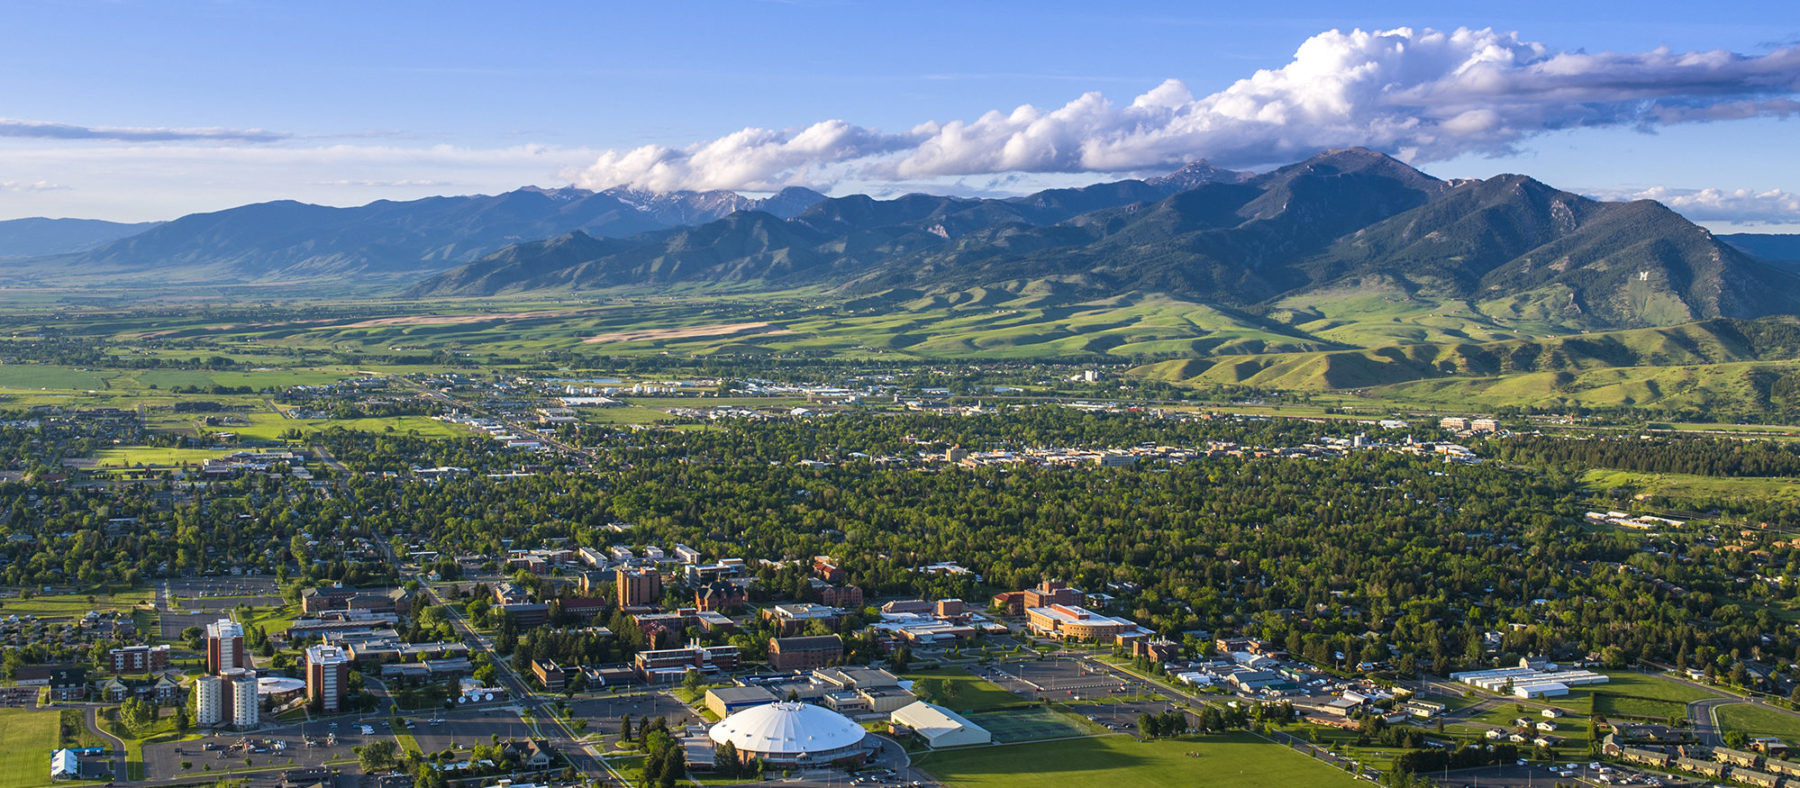
\includegraphics[width=5in,height=\textheight,keepaspectratio]{images/msu-campus.jpg}}
\usepackage{etoolbox}
\makeatletter
\providecommand{\subtitle}[1]{% add subtitle to \maketitle
  \apptocmd{\@title}{\par {\large #1 \par}}{}{}
}
\makeatother
\subtitle{Fall 2025\\
Montana State University}
\author{Melinda Yager\\
Jade Schmidt\\
Stacey Hancock}
\date{}

\begin{document}
\maketitle

\newpage
\thispagestyle{empty}

This resource was developed by Melinda Yager, Jade Schmidt, and Stacey Hancock in 2021 to accompany the online textbook: Hancock, S., Carnegie, N., Meyer, E., Schmidt, J., and Yager, M. (2021). \emph{Montana State Introductory Statistics with R}. Montana State University. \url{https://mtstateintrostats.github.io/IntroStatTextbook/}.

This resource is released under a \href{https://creativecommons.org/licenses/by-nc-sa/4.0/}{Creative Commons BY-NC-SA 4.0} license unless otherwise noted.

\setcounter{tocdepth}{1}
\addtocontents{toc}{\protect\thispagestyle{empty}}
\tableofcontents
\thispagestyle{empty}

\newpage
\setcounter{page}{1}

\chapter*{Preface}\label{preface}
\addcontentsline{toc}{chapter}{Preface}

This coursepack accompanies the textbook for STAT 216: Montana State Introductory Statistics with R, which can be found at \url{https://mtstateintrostats.github.io/IntroStatTextbook/}. The syllabus for the course (including the course calendar), data sets, and links to D2L Brightspace, Gradescope, and the MSU RStudio server can be found on the course webpage: \url{https://math.montana.edu/courses/s216/}.
Other notes and review materials are linked in D2L.

Each of the activities in this workbook is designed to target specific learning outcomes of the course, giving you practice with important statistical concepts in a group setting with instructor guidance. In addition to the in-class activities for the course, video notes are provided to aid in taking notes while you complete the required videos. Bring this workbook with you to class each class period, and take notes in the workbook as you would your own notes. A well-written completed workbook will provide an optimal study guide for exams!

All activities and labs in this coursepack will be completed during class time. Parts of each lab will be turned in on Gradescope. To aid in your understanding, read through the introduction for each activity before attending class each day.

STAT 216 is a 3-credit in-person course. In our experience, it takes six to nine hours per week outside of class to achieve a good grade in this class. By ``good'' we mean at least a C because a grade of D or below does not count toward fulfilling degree requirements. Many of you set your goals higher than just getting a C, and we fully support that. You need roughly nine hours per week to review past activities, read feedback on previous assignments, complete current assignments, and prepare for the next day's class. A typical week in the life of a STAT 216 student looks like:

\begin{itemize}
\tightlist
\item
  \emph{Prior to class meeting}:

  \begin{itemize}
  \tightlist
  \item
    Read assigned sections of the textbook, using the provided reading guides to take notes on the material.
  \item
    Watch the provided videos, taking notes in the coursepack.
  \item
    Read through the introduction to the day's in-class activity.
  \item
    Read through the week's homework assignment and note any questions you may have on the content.
  \end{itemize}
\item
  \emph{During class meeting}:

  \begin{itemize}
  \tightlist
  \item
    Work through the guided activity, in-class activity or weekly lab with your classmates and instructor, taking detailed notes on your answers to each question in the activity.
  \end{itemize}
\item
  \emph{After class meeting}:

  \begin{itemize}
  \tightlist
  \item
    Complete any parts of the activity you did not complete in class.
  \item
    Review the activity solutions in the Math and Stat Center, and take notes on key points.
  \item
    Complete any remaining assigned readings for the week.
  \item
    Complete the week's homework assignment.
  \end{itemize}
\end{itemize}

\nocite{*}

\chapter{Basics of Data and Sampling Methods}\label{basics-of-data-and-sampling-methods}

\section{Vocabulary Review and Key Topics}\label{vocabulary-review-and-key-topics}

At the beginning of each module is a summary of key topics and new vocabulary terms for that module. As you read through the material in the textbook and watch the videos prior to class, look for these terms. Reference the definitions to guide your understanding.

\subsection{Key topics}\label{key-topics}

Module 1 introduces the foundations of data: observational units, types of variables, and how to collect sample data from a population of interest in a way that allows us to generalize our results back to the population.

\subsection{Vocabulary}\label{vocabulary}

\begin{itemize}
\item
  \textbf{Data}: observations used to answer research questions.
\item
  \textbf{Observational units (cases)}: the subjects or entities on which data are collected.

  \begin{itemize}
  \tightlist
  \item
    The rows in a data set represent the observational units.
  \end{itemize}
\item
  \textbf{Sample size}: the number of observational units in a data set, denoted by \(n\).
\item
  \textbf{Variable}: the characteristics collected on each observational unit.
\item
  \textbf{Types of variables}:

  \begin{itemize}
  \item
    \textbf{Categorical}: cases are grouped into categories.
  \item
    \textbf{Quantitative}: numerical measurements, where performing arithmetic operations makes sense.
  \end{itemize}
\item
  \textbf{Target population}: group of observational units of interest.
\item
  \textbf{Sample}: subset of the population.
\item
  \textbf{Sampling methods}:

  \begin{itemize}
  \item
    \textbf{Unbiased sampling method (e.g., a random sample)}: on average, the sample will be representative of the target population; all observational units in the target population have the same chance of being selected.
  \item
    \textbf{Biased sampling method (e.g., convenience sample)}: on average, the sample will not be representative of the target population; some part of the target population will be over- or under-represented.
  \end{itemize}
\item
  \textbf{Type of sampling bias}:

  \begin{itemize}
  \item
    \textbf{Selection bias}: method of sampling is biased; some part of the target population is over- or under-represented.
  \item
    \textbf{Non-response bias}: part of a pre-selected sample does not respond or cannot be reached.
  \item
    \textbf{Response bias}: responses are not truthful (poor/leading question phrasing, social desirability).
  \end{itemize}
\end{itemize}

\newpage

\begin{itemize}
\item
  \textbf{Generalization}: to what group of observational units can the results be applied to?

  \begin{itemize}
  \item
    If an unbiased method of selection was used and there is no non-response or response bias, we can generalize the results to the target population.
  \item
    If a biased method of selection was used or if non-response or response bias is present, we can only generalize the result to the sample or similar observational units.
  \end{itemize}
\end{itemize}

\newpage

\section{Activity 1: Intro to Data Analysis and Sampling Bias}\label{activity-1-intro-to-data-analysis-and-sampling-bias}

\setstretch{1}

\subsection{Learning outcomes}\label{learning-outcomes}

\begin{itemize}
\item
  Identify observational units, variables, and variable types in a statistical study.
\item
  Creating a data set
\item
  Identify biased sampling methods.
\end{itemize}

\subsection{Terminology review}\label{terminology-review}

Statistics is the study of how best to collect, analyze, and draw conclusions from data. In the next few days of class, we will learn the building blocks of the semester. This week in class you will be introduced to the following terms:

\begin{itemize}
\item
  Observational units or cases
\item
  Variables: categorical or quantitative
\item
  Selection bias
\item
  Response bias
\item
  Non-response bias
\end{itemize}

For more on these concepts, read Chapter 1 and 2 in the textbook.

\subsection*{Notes on Observational Units and Variables}\label{notes-on-observational-units-and-variables}
\addcontentsline{toc}{subsection}{Notes on Observational Units and Variables}

\vspace{4in}

\subsubsection*{Further analysis of class data set}\label{further-analysis-of-class-data-set}
\addcontentsline{toc}{subsubsection}{Further analysis of class data set}

\begin{enumerate}
\def\labelenumi{\arabic{enumi}.}
\tightlist
\item
  What are the observational units or cases for the data collected in class on day 1?
\end{enumerate}

\vspace{0.3in}

\begin{enumerate}
\def\labelenumi{\arabic{enumi}.}
\setcounter{enumi}{1}
\tightlist
\item
  How many observations are reported in the data set? This is the \textbf{sample size}.
\end{enumerate}

\vspace{0.3in}

\begin{enumerate}
\def\labelenumi{\arabic{enumi}.}
\setcounter{enumi}{2}
\tightlist
\item
  The header for each column in the data set describes each variable measured on the observational unit. For each column of data, fill in the following table identifying the type of each variable.
\end{enumerate}

\begin{itemize}
\item
  If the variable is categorical, indicate in column 3 whether the variable is binary.
\item
  If the variable is quantitative, indicate in column 4 the units of measure used.
\end{itemize}

\begin{center}
\begin{tabular}{|l|p{1.5in}|p{0.5in}|p{0.5in}|} \hline
Column & Type of Variable & Binary? & Units? \\ \hline
Major & & &\\
& & & \\ \hline
Residency & & & \\
& & & \\ \hline
Num Credits & & & \\
& & & \\ \hline
Dominant hand & & & \\
& & & \\ \hline
Hand Span & & & \\
& & & \\ \hline
Grip strength dominant hand & & & \\
& & & \\ \hline
Grip strength non-dominant hand & & & \\
& & & \\ \hline
\end{tabular}
\end{center}

\begin{enumerate}
\def\labelenumi{\arabic{enumi}.}
\setcounter{enumi}{3}
\tightlist
\item
  Review the completed data set with your class. Remember that when creating a data set for use in R it is important to use single words or an underscore between words. Each outcome must be written the same way each time to have consistency between responses. Do not include units of measure in the data set when reporting numerical values. Write down some issues found with the created class data set.
\end{enumerate}

\vspace{2.5in}

\subsection*{Notes on Sampling Methods and Types of bias}\label{notes-on-sampling-methods-and-types-of-bias}
\addcontentsline{toc}{subsection}{Notes on Sampling Methods and Types of bias}

\vspace{5in}

\newpage

\subsubsection*{Types of bias}\label{types-of-bias}
\addcontentsline{toc}{subsubsection}{Types of bias}

Complete Q5 together as a class:

\begin{enumerate}
\def\labelenumi{\arabic{enumi}.}
\setcounter{enumi}{4}
\item
  A television station is interested in predicting whether or not local voters will pass a referendum to legalize marijuana for adult. The TV station asks its viewers to phone in and indicate whether they are in favor or opposed to the referendum. Of the 2241 viewers who phoned in, forty-five percent were opposed to legalizing marijuana.
  \vspace{0.1in}

  Sample size:
  \vspace{0.3in}

  Observational units sampled:
  \vspace{0.3in}

  Target population:
  \vspace{0.3in}

  Justify why there is selection bias in this study.
  \vspace{0.5in}
\item
  To determine if the proportion of out-of-state undergraduate students at Montana State University has increased in the last 10 years, a statistics instructor sent an email survey to 500 randomly selected current undergraduate students. One of the questions on the survey asked whether they had in-state or out-of-state residency. She only received 378 responses.
  \vspace{0.1in}

  Sample size:
  \vspace{0.3in}

  Observational units sampled:
  \vspace{0.3in}

  Target population:
  \vspace{0.3in}

  Justify why there is non-response bias in this study.
  \vspace{0.5in}
\end{enumerate}

\newpage

\begin{enumerate}
\def\labelenumi{\arabic{enumi}.}
\setcounter{enumi}{6}
\item
  To gauge the interest of Bozeman City Voters in a new swimming pool, a local organization stood outside of the Bogart Pool in Bozeman, MT, during open hours. One of the questions they asked was, ``Since the Bogart Pool is in such bad repair, don't you agree that the city should fund a new pool?''
  \vspace{0.1in}

  Sample size:
  \vspace{0.3in}

  Observational units sampled:
  \vspace{0.3in}

  Target population:
  \vspace{0.3in}

  Justify why there is response bias in this study.
  \vspace{0.5in}

  Justify why there is selection bias in this study.
  \vspace{0.5in}
\end{enumerate}

\subsection{Take-home messages}\label{take-home-messages}

\begin{enumerate}
\def\labelenumi{\arabic{enumi}.}
\item
  There are two types of variables: categorical (groups) and quantitative (numerical measures).
\item
  We will learn more about summarizing variable later in the semester. Categorical variables are summarized by calculating a proportion from the data and quantitative variables are summarized by finding the mean and the standard deviation.
\item
  There are three types of bias to be aware of when designing a sampling method: selection bias, non-response bias, and response bias.
\end{enumerate}

\subsection{Additional notes}\label{additional-notes}

Use this space to summarize your thoughts and take additional notes on today's activity and material covered, and to write down the names and contact information of your teammates.

\newpage

\section{Activity 2: American Indian Address}\label{activity-2-american-indian-address}

\setstretch{1}

\subsection{Learning outcomes}\label{learning-outcomes-1}

\begin{itemize}
\item
  Explain why a sampling method is unbiased or biased.
\item
  Identify biased sampling methods.
\item
  Explain the purpose of random selection and its effect on generalization.
\end{itemize}

\subsection{Terminology review}\label{terminology-review-1}

In this activity, we will examine unbiased and biased methods of sampling. Some terms covered in this activity are:

\begin{itemize}
\item
  Random sample
\item
  Unbiased vs biased methods of selection
\item
  Generalization
\end{itemize}

To review these concepts, see Chapter 2 in the textbook.

\subsection{Class Preparation}\label{class-preparation}

Prior to the next class, complete questions 1--3.

\subsection{American Indian Address}\label{american-indian-address}

For this activity, you will read a speech given by Jim Becenti, a member of the Navajo American Indian tribe, who spoke about the employment problems his people faced at an Office of Indian Affairs meeting in Phoenix, Arizona, on January 30, 1947 (Moquin and Van Doren 1973). His speech is below:

\textbf{It is hard for us to go outside the reservation where we meet strangers. I have been off the reservation ever since I was sixteen. Today I am sorry I quit the Santa Fe {[}Railroad{]}. I worked for them in 1912--13. You are enjoying life, liberty, and happiness on the soil the American Indian had, so it is your responsibility to give us a hand, brother. Take us out of distress. I have never been to vocational school. I have very little education. I look at the white man who is a skilled laborer. When I was a young man I worked for a man in Gallup as a carpenter's helper. He treated me as his own brother. I used his tools. Then he took his tools and gave me a list of tools I should buy and I started carpentering just from what I had seen. We have no alphabetical language.}

\textbf{We see things with our eyes and can always remember it. I urge that we help my people to progress in skilled labor as well as common labor. The hope of my people is to change our ways and means in certain directions, so they can help you someday as taxpayers. If not, as you are going now, you will be burdened the rest of your life. The hope of my people is that you will continue to help so that we will be all over the United States and have a hand with you, and give us a brotherly hand so we will be happy as you are. Our reservation is awful small. We did not know the capacity of the range until the white man come and say ``you raise too much sheep, got to go somewhere else,'' resulting in reduction to a skeleton where the Indians can't make a living on it. For eighty years we have been confused by the general public, and what is the condition of the Navajo today? Starvation! We are starving for education. Education is the main thing and the only thing that is going to make us able to compete with you great men here talking to us.}

\subsubsection*{By eye selection}\label{by-eye-selection}
\addcontentsline{toc}{subsubsection}{By eye selection}

\begin{enumerate}
\def\labelenumi{\arabic{enumi}.}
\tightlist
\item
  Circle ten words in Jim Becenti's speech which are a representative sample of the length of words in the entire text. Describe your method for selecting this sample.
\end{enumerate}

\vspace{0.3in}

\begin{enumerate}
\def\labelenumi{\arabic{enumi}.}
\setcounter{enumi}{1}
\tightlist
\item
  Fill in the table below with your selected words from the previous question and the length of each word (number of letters/digits in the word):
  \vspace{1mm}
\end{enumerate}

\begin{center}
\begin{tabular}{|l|p{3in}|p{1in}|} \hline
Observation & Word & Length  \\ \hline
1 & & \\ 
& & \\ \hline
2 & & \\ 
& & \\ \hline
3 & & \\ 
& & \\ \hline
4 & & \\ 
& & \\ \hline
5 & & \\ 
& & \\ \hline
6 & & \\ 
& & \\ \hline
7 & & \\
& & \\ \hline
8 & & \\ 
& & \\ \hline
9 & & \\ 
& & \\ \hline
10 & & \\ 
& & \\ \hline
\end{tabular}
\end{center}

\begin{enumerate}
\def\labelenumi{\arabic{enumi}.}
\setcounter{enumi}{2}
\tightlist
\item
  Calculate the mean (average) word length in your selected sample. Is this value a parameter or a statistic?\\
  \vspace{0.3in}
\end{enumerate}

\subsection*{Notes on sampling}\label{notes-on-sampling}
\addcontentsline{toc}{subsection}{Notes on sampling}

\vspace{5in}

\subsection{Class Activity}\label{class-activity}

\begin{enumerate}
\def\labelenumi{\arabic{enumi}.}
\tightlist
\item
  Report your mean word length from question3 to your instructor. Your instructor will create a visualization of the distribution of results generated by your class. Draw a picture of the plot here. Include a descriptive \(x\)-axis label. Report the mean and standard deviation of the sample mean word lengths.
\end{enumerate}

\vspace{2in}

\newpage

The plot created in question 1 is a sampling distribution of statistics. This sampling distribution plots the mean word length from many samples taken from the population of words.

\begin{enumerate}
\def\labelenumi{\arabic{enumi}.}
\setcounter{enumi}{1}
\item
  The true mean word length of the population of all 359 words in the speech is 3.95 letters. Is this value a parameter or a statistic?\\
  \vspace{0.2in}

  Where does the value of 3.95 fall in the plot given? Near the center of the distribution? In the tails of the distribution?
  \vspace{0.3in}
\item
  Based on the class discussion, would you say the sampling method used (``by-eye'' selection) by the class is biased or unbiased? Justify your answer.\\
  \vspace{0.5in}
\item
  If the sampling method is biased, what type of sampling bias (selection, response, non-response) is present? What is the direction of the bias, i.e., does the method tend to overestimate or underestimate the population mean word length?
  \vspace{0.5in}
\end{enumerate}

\subsubsection*{Random selection}\label{random-selection}
\addcontentsline{toc}{subsubsection}{Random selection}

Suppose instead of attempting to select a representative sample by eye (which did not work), each student used a random number generator to select a simple random sample of 10 words. A \textbf{simple random sample} relies on a random mechanism to choose a sample, without replacement, from the population, such that every sample of size 10 is equally likely to be chosen.

To use a random number generator to select a simple random sample, you first need a numbered list of all the words in the population, called a \textbf{sampling frame}. You can then generate 10 random numbers from the numbers 1 to 359 (the number of words in the population), and the chosen random numbers correspond to the chosen words in your sample.

\begin{enumerate}
\def\labelenumi{\arabic{enumi}.}
\setcounter{enumi}{4}
\tightlist
\item
  Use the random number generator at \url{https://istats.shinyapps.io/RandomNumbers/} to select a simple random sample from the population of all 359 words in the speech.
\end{enumerate}

\begin{itemize}
\item
  Set ``Choose Minimum'' to 1 and ``Choose Maximum'' to 359 to represent the 359 words in the population (the sampling frame).
\item
  Set ``How many numbers do you want to generate?'' to 10 and ensure the ``No'' option is selected under ``Sample with Replacement?''
\item
  Click ``Generate''.
\end{itemize}

Fill in the table on the next page with the random numbers selected and use the Becenti.csv data file found on D2L to determine each number's corresponding word and word length (number of letters/digits in the word):

\begin{center}
\begin{tabular}{|l|l|p{1in}|} \hline
Observation & Number & Length  \\ \hline
1 & & \\ 
& & \\ \hline
2 & & \\ 
& & \\ \hline
3 & & \\ 
& & \\ \hline
4 & & \\ 
& & \\ \hline
5 & & \\ 
& & \\ \hline
6 & & \\ 
& & \\ \hline
7 & & \\
& & \\ \hline
8 & & \\ 
& & \\ \hline
9 & &\\ 
& & \\ \hline
10 & & \\ 
& & \\ \hline
\end{tabular}
\end{center}

\begin{enumerate}
\def\labelenumi{\arabic{enumi}.}
\setcounter{enumi}{5}
\item
  Calculate the mean word length in your selected sample in question 5. Is this value a parameter or a statistic?
  \vspace{0.3in}
\item
  Report your mean word length in the Google sheet. Your instructor will create a visualization of the distribution of results generated by your class. Draw a picture of the plot here. Include a descriptive \(x\)-axis label. Report the mean and standard deviation of the samples.
\end{enumerate}

\vspace{2.25in}

\begin{enumerate}
\def\labelenumi{\arabic{enumi}.}
\setcounter{enumi}{7}
\tightlist
\item
  Where does the value 3.95, the true mean word length, fall in the distribution given? Near the center of the distribution? In the tails of the distribution? Circle this value on the provided distribution.
  \vspace{0.3in}
\end{enumerate}

\newpage

One set of randomly generated sample mean word lengths from a single class may not be large enough to visualize the distribution results. Let's have a computer generate 1,000 sample mean word lengths for us.

The following plot illustrates a sampling distribution of 1000 samples of size 10 selected at random from the sample.

\begin{center}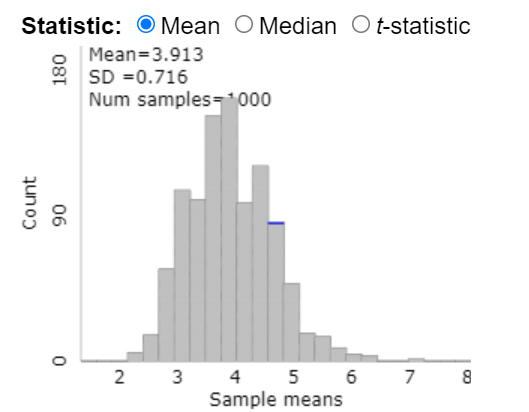
\includegraphics[width=0.75\linewidth]{images/bencenti_sampling10} \end{center}

\begin{enumerate}
\def\labelenumi{\arabic{enumi}.}
\setcounter{enumi}{8}
\item
  What is the center value (mean) of the distribution displayed above?
  \vspace{0.3in}
\item
  Explain why the sampling method of using a random number generator to generate a sample is a ``better'' method than choosing 10 words ``by eye''.
  \vspace{0.8in}
\item
  Is random selection an unbiased method of selection? Explain your answer. Be sure to reference the plot from before Q15.
  \vspace{0.5in}
\end{enumerate}

\newpage

\subsection*{Effect of sample size}\label{effect-of-sample-size}
\addcontentsline{toc}{subsection}{Effect of sample size}

We will now consider the impact of sample size.

\begin{enumerate}
\def\labelenumi{\arabic{enumi}.}
\setcounter{enumi}{11}
\tightlist
\item
  First, consider if each student had selected 30 words, instead of 10, by eye. Do you think this would make the plot from the previous activity centered on 3.95 (the true mean word length)? Explain your answer.
  \vspace{0.4in}
\end{enumerate}

\newpage

Now we will select 30 words instead of 10 words at random. The following plot illustrates a sampling distribution of 1000 samples of size 30 selected at random from the sample.

\begin{center}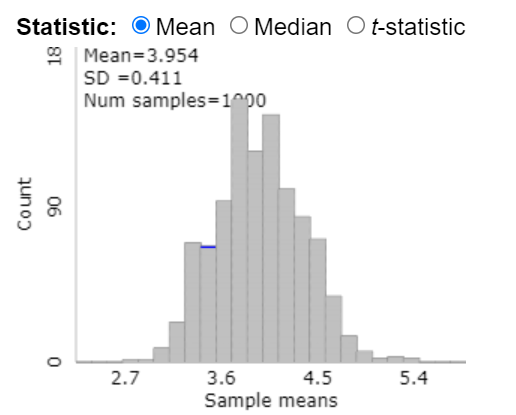
\includegraphics[width=0.75\linewidth]{images/bencenti_sampling30} \end{center}

\begin{enumerate}
\def\labelenumi{\arabic{enumi}.}
\setcounter{enumi}{12}
\item
  Compare the values of the standard deviation of the plots before question 9 and before question 13. Which plot shows the smallest standard deviation?
  \vspace{0.4in}
\item
  Using the evidence from your simulations, answer the following research questions:
\end{enumerate}

\rgi Does changing the sample size impact whether the sample estimates are unbiased? Explain your answer.
\vspace{0.5in}

\rgi Does changing the sample size impact the variability (spread) of sample estimates? Explain your answer
\vspace{0.5in}

\begin{enumerate}
\def\labelenumi{\arabic{enumi}.}
\setcounter{enumi}{14}
\tightlist
\item
  What is the purpose of random selection of a sample from the population?
\end{enumerate}

\vspace{0.8in}

\subsection{Take-home messages}\label{take-home-messages-1}

\begin{enumerate}
\def\labelenumi{\arabic{enumi}.}
\item
  When we use a biased method of selection, we will over or underestimate the parameter.
\item
  If the sampling method is biased, inferences made about the population based on a sample estimate will not be valid.
\item
  Random selection is an unbiased method of selection.
\item
  To determine if a sampling method is biased or unbiased, we compare the distribution of the estimates to the true value. We want our estimate to be on target or unbiased. When using unbiased methods of selection, the mean of the distribution matches or is very similar to our true parameter.
\item
  Random selection eliminates selection bias. However, random selection will not eliminate response or non-response bias.
\item
  The larger the sample size, the more similar (less variable) the statistics will be from different samples.
\item
  Sample size has no impact on whether a \emph{sampling method} is biased or not. Taking a larger sample using a biased method will still result in a sample that is not representative of the population.
\end{enumerate}

\subsection{Additional notes}\label{additional-notes-1}

Use this space to summarize your thoughts and take additional notes on today's activity and material covered.

\newpage

\chapter{Probability}\label{probability}

\section{Vocabulary Review and Key Topics}\label{vocabulary-review-and-key-topics-1}

\subsection{Key topics}\label{key-topics-1}

Module 2 introduces the concept of probability as a long-run relative frequency and demonstrates how to use hypothetical two-way tables to set up a probability problem and solve for unconditional and conditional probabilities.

\subsection{Vocabulary}\label{vocabulary-1}

\begin{itemize}
\item
  \textbf{Probability} (of an event): the long-run proportion of times the event would occur if the random process were repeated indefinitely (under identical conditions).
\item
  \textbf{Conditional probability} (of an event \emph{given} another event): probability of an event calculated dependent on another event having occurred.
\item
  \textbf{Probability notation}:

  \begin{itemize}
  \item
    \(P(A)\): the probability of event \(A\).

    \begin{itemize}
    \tightlist
    \item
      This is the probability of a single event, \emph{unconditional} probability calculated out of the overall population.
    \end{itemize}
  \item
    \(P(A^C)\): the probability of the \textbf{complement} of event \(A\), or ``\(A\) complement''.

    \begin{itemize}
    \item
      This is the probability of the opposite of event \(A\), or ``not \(A\)''.
    \item
      \(P(A^C) = 1 - P(A)\)
    \end{itemize}
  \item
    \(P(A\text{ and }B)\): the probability of event \(A\) and \(B\).

    \begin{itemize}
    \tightlist
    \item
      The is the probability of an ``and'' event, \emph{unconditional} probability calculated out of the overall population.
    \end{itemize}
  \item
    \(P(A|B)\): the probability of event \(A\) given (conditional on) event \(B\).

    \begin{itemize}
    \tightlist
    \item
      This is a \emph{conditional} probability calculated out of the total population for which event \(B\) occurred.
    \end{itemize}
  \end{itemize}
\end{itemize}

\newpage

\section{Activity 3: Probability Studies}\label{activity-3-probability-studies}

\setstretch{1}

\subsection{Learning outcomes}\label{learning-outcomes-2}

\begin{itemize}
\item
  Recognize and simulate probabilities as long-run frequencies.
\item
  Construct two-way tables to evaluate conditional probabilities.
\end{itemize}

\subsection{Terminology review}\label{terminology-review-2}

In today's activity, we will cover two-way tables and probability. Some terms covered in this activity are:

\begin{itemize}
\item
  Proportions
\item
  Probability
\item
  Conditional probability
\item
  Two-way tables
\end{itemize}

To review these concepts, see Chapter 23 in the textbook.

\subsection*{Notes on probability}\label{notes-on-probability}
\addcontentsline{toc}{subsection}{Notes on probability}

The probability of an event is the long-run proportion of times the event would occur if the random process were repeated indefinitely (under identical conditions).

To calculate the probability of an event happening:

\[\text{probability} = \frac{\text{number of ways an event can happen}}{\text{total number of possible outcomes}}\]

For example, to calculate the probability of a coin flip landing on heads; there are only two outcomes (heads or tails) and only one possibility way to land on heads.

\[P(heads) = \frac{1}{2} = 0.5\]
The figure below shows the long-run proportion of times a simulated coin flip lands on heads on the y-axis, and the number of tosses on the x-axis. Notice how the long-run proportion starts converging to 0.5 as the number of tosses increases.

\begin{figure}

{\centering 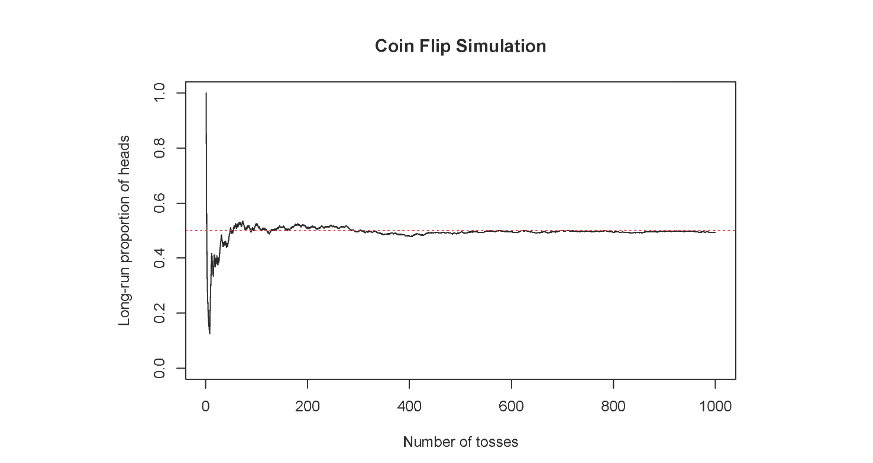
\includegraphics[width=0.65\linewidth]{images/coinsim} 

}

\end{figure}

In today's activity we will discuss the probability of a single event, the probability of an ``and'' event, and the probability of a conditional event.

\subsubsection*{Probability notation}\label{probability-notation}
\addcontentsline{toc}{subsubsection}{Probability notation}

We will use the notation P(event) to represent the probability of an event and use letters to represent events. The following are notations for different probabilities where we are discussing event A and event B:

\begin{itemize}
\item
  \(P(A)\) represents the probability of event A
\item
  \(P(A^C)\) represents the probability of the complement of event A

  \begin{itemize}
  \tightlist
  \item
    \(P(A^C) = 1 - P(A)\)
  \end{itemize}
\item
  \(P(A and B)\) represents the probability of events A and B
\item
  \(P(A|B)\) represents the probability of event A given event B
\item
  \(P(B|A)\) represents the probability of event B given event A
\end{itemize}

\subsubsection{Probability questions}\label{probability-questions}

For the beginning of this activity we will start with discussing the probabilities associated with drawing a card from a standard card deck. In a card deck there are:

\begin{itemize}
\item
  52 cards
\item
  Half are red, half are black
\item
  Four suits: spades, hearts, diamonds, and clubs
\item
  Each suit has 13 cards: cards 2--10, ace, jack, queen, and king
\item
  Let A represent the event that a card is an ace
\item
  Let B represent the event that a card is red
\end{itemize}

To find the probability of selecting an ace, first start with determining how many aces are possible (four) and how many cards will we select from (total of 52).

\vspace{1in}

Find the probability of selecting a card that is not an ace. This is the complement of event A.

\vspace{1in}

Find the probability of selecting a red ace.

\vspace{1in}

Find the probability of selecting an ace given that the card is red.

\vspace{1in}

If a card drawn is an ace, what is the probability the card drawn is red.

\vspace{1in}

\subsection{Calculating probabilities from a two-way table}\label{calculating-probabilities-from-a-two-way-table}

\begin{enumerate}
\def\labelenumi{\arabic{enumi}.}
\tightlist
\item
  In 2014, the website FiveThirtyEight examined the works of Bob Ross to see what trends could be found. They determined that of all the paintings he created, 95\% of them contained at least one ``happy tree.'' Of those works with a happy tree, 43\% contained at least one ``almighty mountain.'' Of the paintings that did not have at least one happy tree, only 10\% contained at least one almighty mountain.
  \vspace{1mm}
\end{enumerate}

Let \(A\) = Bob Ross painting contains a happy tree, and \(B\) = Bob Ross painting contains an almighty mountain
\vspace{0.1in}

\begin{center}
\begin{tabular}{|c|c|c|c|} \hline
\hspace{0.8in} & \hspace{0.25in}  $A$ \hspace{.25in} & \hspace{0.25in} $A^C$ \hspace{0.25in} & \hspace{0.25in} Total \hspace{0.25in} \\ \hline
 $B$ & 40850 & 500 & 41350 \\ \hline
 $B^C$ & 54150 & 4500 & 58650 \\ \hline
Total & 95000 & 5000 & 100000 \\ \hline
\end{tabular}
\end{center}
\vspace{.1in}

\begin{enumerate}
\def\labelenumi{\alph{enumi}.}
\tightlist
\item
  What is the probability that a randomly selected Bob Ross painting contains both a ``happy tree'' and an ``almighty mountain''? Use appropriate probability notation.
\end{enumerate}

\vspace{0.5in}

\begin{enumerate}
\def\labelenumi{\alph{enumi}.}
\setcounter{enumi}{1}
\tightlist
\item
  What is the probability that a selected Bob Ross painting without an ``almighty mountain'' contains a ``happy tree.'' Use appropriate probability notation.
\end{enumerate}

\vspace{0.5in}

\begin{enumerate}
\def\labelenumi{\alph{enumi}.}
\setcounter{enumi}{2}
\tightlist
\item
  What is the probability that a selected Bob Ross painting does not contain a ``happy tree'' given it does not contain an ``almighty mountain''. Use appropriate probability notation.
\end{enumerate}

\vspace{0.55in}

\newpage

\begin{enumerate}
\def\labelenumi{\arabic{enumi}.}
\setcounter{enumi}{1}
\item
  A recent study of population decline of white-tailed deer in Wyoming due to chronic wasting disease (Edmunds 2016) (CWD) reported that 35.4\% of white-tailed deer have CWD. The survival rate of deer with CWD is 39.6\% and the survival rate of deer without CWD is 80.1\%.\\
  \vspace{1mm}

  Let \(A\) = the event a deer has CWD, and \(B\) = the event the deer survives.
  \vspace{0.1in}

  \begin{enumerate}
  \def\labelenumii{\alph{enumii}.}
  \item
    Identify what each numerical value given in the problem represents in probability notation.
    \vspace{.1in}

    0.354 =\\
    \vspace{.1in}

    0.396 =\\
    \vspace{.1in}

    0.801 =\\
    \vspace{.1in}
  \item
    Create a hypothetical two-way table to represent the situation.
  \end{enumerate}
\end{enumerate}

\begin{center}
\begin{tabular}{|c|c|c|c|} \hline
\hspace{0.8in} & \hspace{0.35in} $A$ \hspace{.35in} & \hspace{0.35in} $A^C$  \hspace{0.35in} & \hspace{0.3in} Total \hspace{0.3in} \\ 
& & & \\ \hline
$B$& & & \\ 
& & & \\ \hline
$B^C$& & & \\ 
& & & \\ \hline
Total & & & 100,000 \\ 
& & & \\ \hline
\end{tabular}
\end{center}
\vspace{.1in}

\begin{enumerate}
\def\labelenumi{\alph{enumi}.}
\setcounter{enumi}{2}
\item
  Find \(P(A \mbox{ and } B)\). What does this probability represent in the context of the problem?
  \vspace{.8in}
\item
  Find the probability that a deer that has CWD does not survive. What is the notation used for this probability?
  \vspace{.8in}
\item
  What is the probability that a deer does not survive given they do not have CWD? What is the notation used for this probability?
\end{enumerate}

\newpage

\begin{enumerate}
\def\labelenumi{\arabic{enumi}.}
\setcounter{enumi}{2}
\item
  Since the early 1980s, the rapid antigen detection test (RADT) of group A \emph{streptococci} has been used to detect strep throat. A recent study of the accuracy of this test shows that the \textbf{sensitivity}, the probability of a positive RADT given the person has strep throat, is 86\% in children, while the \textbf{specificity}, the probability of a negative RADT given the person does not have strep throat, is 92\% in children. The \textbf{prevalence}, the probability of having group A strep, is 37\% in children. (Stewart et al. 2014)
  \vspace{1mm}

  Let \(A\) = the event the child has strep throat, and \(B\) = the event the child has a positive RADT.
  \vspace{0.1in}

  \begin{enumerate}
  \def\labelenumii{\alph{enumii}.}
  \item
    Identify what each numerical value given in the problem represents in probability notation.
    \vspace{.1in}

    0.86 =\\
    \vspace{.1in}

    0.92 =\\
    \vspace{.1in}

    0.37 =\\
    \vspace{.1in}
  \item
    Create a hypothetical two-way table to represent the situation.
  \end{enumerate}
\end{enumerate}

\begin{center}
\begin{tabular}{|c|c|c|c|} \hline
\hspace{0.8in} & \hspace{0.35in} $A$ \hspace{.35in} & \hspace{0.35in} $A^C$  \hspace{0.35in} & \hspace{0.3in} Total \hspace{0.3in} \\ 
& & & \\ \hline
$B$& & & \\ 
& & & \\ \hline
$B^C$& & & \\ 
& & & \\ \hline
Total & & & 100,000 \\ 
& & & \\ \hline
\end{tabular}
\end{center}
\vspace{.1in}

\begin{enumerate}
\def\labelenumi{\alph{enumi}.}
\setcounter{enumi}{2}
\item
  Find \(P(B)\). What does this probability represent in the context of the problem?
  \vspace{.8in}
\item
  Find the probability that a child with a positive RADT actually has strep throat. What is the notation used for this probability?
  \vspace{.8in}
\item
  What is the probability that a child does not have strep given that they have a positive RADT? What is the notation used for this probability?
\end{enumerate}

\vspace{0.8in}

\subsection{Take home messages}\label{take-home-messages-2}

\begin{enumerate}
\def\labelenumi{\arabic{enumi}.}
\item
  Conditional probabilities are calculated dependent on a second variable. In probability notation, the variable following \texttt{\textbar{}} is the variable on which we are conditioning. The denominator used to calculate the probability will be the total for the variable on which we are conditioning.
\item
  When creating a two-way table we typically want to put the explanatory variable on the columns of the table and the response variable on the rows.
\item
  To fill in the two-way table, always start with the unconditional variable in the total row or column and then use the conditional probabilities to fill in the interior cells.
\end{enumerate}

\subsection{Additional notes}\label{additional-notes-2}

Use this space to summarize your thoughts and take additional notes on today's activity and material covered.

\newpage

\chapter{Exploring Categorical Data: Exploratory Data Analysis and Inference using Simulation-based Methods}\label{exploring-categorical-data-exploratory-data-analysis-and-inference-using-simulation-based-methods}

\section{Vocabulary Review and Key Topics}\label{vocabulary-review-and-key-topics-2}

Review the Golden Ticket posted in the resources at the end of the coursepack for a summary of a single categorical variable.

\subsection{Key topics}\label{key-topics-2}

Module 3 introduces the steps of the statistical investigation process. We conduct \textbf{exploratory data analysis} (summary statistics and plots) and simulation-based \textbf{inference} (hypothesis testing and confidence intervals) in the single categorical variable (one proportion) scenario.

\begin{itemize}
\item
  Notation for a sample proportion: \(\hat{p}\)
\item
  Notation for a population proportion: \(\pi\)
\item
  Types of plots for a single categorical variable:

  \begin{itemize}
  \item
    Frequency bar plot
  \item
    Relative frequency bar plot
  \end{itemize}
\end{itemize}

Exploratory data analysis is step 3 of the statistical investigation process. We will then use simulation-based methods \textbf{to find evidence of an effect by finding a p-value} and \textbf{estimating how large the effect is by creating a confidence interval} in the one proportion (one categorical variable) scenario. These are steps 4 and 5 from the steps of the statistical investigation process.

\subsubsection*{Steps of the statistical investigation process}\label{steps-of-the-statistical-investigation-process}
\addcontentsline{toc}{subsubsection}{Steps of the statistical investigation process}

As we move through the semester we will work through the six steps of the statistical investigation process.

\begin{enumerate}
\def\labelenumi{\arabic{enumi}.}
\item
  Ask a research question.
\item
  Design a study and collect data.
\item
  Summarize and visualize the data.
\item
  Use statistical analysis methods to draw inferences from the data.
\item
  Communicate the results and answer the research question.
\item
  Revisit and look forward.
\end{enumerate}

\subsection{Vocabulary}\label{vocabulary-2}

\begin{itemize}
\item
  \textbf{Summary measure}: a numerical quantity that summarizes data. Summary measures covered in STAT 216 include: single proportion, difference in proportions, single mean, paired mean difference, difference in means, correlation, and slope of a regression line.

  \begin{itemize}
  \tightlist
  \item
    For a single categorical variable, a proportion is calculated.
  \end{itemize}
\item
  \textbf{Summary statistic (point estimate)}: the value of a numerical summary measure computed from \emph{sample} data.

  \begin{itemize}
  \item
    To interpret in context include:

    \begin{itemize}
    \item
      Summary measure (in context)
    \item
      Value of the statistic
    \end{itemize}
  \end{itemize}
\item
  \textbf{Parameter of interest}: a numerical summary measure of the entire \emph{population} in which we are interested.

  \begin{itemize}
  \item
    The value of the parameter of interest is unknown (unless we have access to the entire population).
  \item
    To write in context:

    \begin{itemize}
    \item
      Population word (true, long-run, population)
    \item
      Summary measure (depends on the type of data)
    \item
      Context

      \begin{itemize}
      \item
        Observational units
      \item
        Variable(s)
      \end{itemize}
    \end{itemize}
  \end{itemize}
\item
  For a single categorical variable, the category that we are counting the proportion of is generically called a ``\textbf{success}'', with categories not a success labeled ``\textbf{failure}''. Thus, a sample proportion is the ``proportion of successes'' in the sample: the total number of successes divided by the sample size (\(n\)).
\end{itemize}

\subsubsection*{Plotting one categorical variable}\label{plotting-one-categorical-variable}
\addcontentsline{toc}{subsubsection}{Plotting one categorical variable}

\begin{itemize}
\item
  \textbf{Frequency bar plot}: plots the count (frequency) of observational units in each level of a categorical variable. R code to create a frequency bar plot:

\begin{Shaded}
\begin{Highlighting}[]
\NormalTok{object }\SpecialCharTok{\%\textgreater{}\%} \CommentTok{\# Data set piped into...}
\FunctionTok{ggplot}\NormalTok{(}\FunctionTok{aes}\NormalTok{(}\AttributeTok{x =}\NormalTok{ variable)) }\SpecialCharTok{+}   \CommentTok{\# This specifies the variable}
\FunctionTok{geom\_bar}\NormalTok{(}\AttributeTok{stat =} \StringTok{"count"}\NormalTok{) }\SpecialCharTok{+}  \CommentTok{\# Tell it to make a bar plot}
\FunctionTok{labs}\NormalTok{(}\AttributeTok{title =} \StringTok{"Don\textquotesingle{}t forget to title your plot!"}\NormalTok{,  }
   \CommentTok{\# Give your plot a title}
   \AttributeTok{x =} \StringTok{"x{-}axis label"}\NormalTok{,   }\CommentTok{\# Label the x axis}
   \AttributeTok{y =} \StringTok{"Frequency"}\NormalTok{)  }\CommentTok{\# Label the y axis}
\end{Highlighting}
\end{Shaded}
\item
  \textbf{Relative frequency bar plot}: plots the proportion (relative frequency) of observational units in each level of a categorical variable. R code to create a relative frequency bar plot:

\begin{Shaded}
\begin{Highlighting}[]
\NormalTok{object }\SpecialCharTok{\%\textgreater{}\%} \CommentTok{\# Data set piped into...}
\FunctionTok{ggplot}\NormalTok{(}\FunctionTok{aes}\NormalTok{(}\AttributeTok{x =}\NormalTok{ variable)) }\SpecialCharTok{+}   \CommentTok{\# This specifies the variable}
\FunctionTok{geom\_bar}\NormalTok{(}\FunctionTok{aes}\NormalTok{(}\AttributeTok{y =} \FunctionTok{after\_stat}\NormalTok{(prop), }\AttributeTok{group =} \DecValTok{1}\NormalTok{)) }\SpecialCharTok{+}  \CommentTok{\# Tell it to make a bar plot with proportions}
\FunctionTok{labs}\NormalTok{(}\AttributeTok{title =} \StringTok{"Don\textquotesingle{}t forget to title your plot!"}\NormalTok{,  }
   \CommentTok{\# Give your plot a title}
   \AttributeTok{x =} \StringTok{"x{-}axis label"}\NormalTok{,   }\CommentTok{\# Label the x axis}
   \AttributeTok{y =} \StringTok{"Relative Frequency"}\NormalTok{)  }\CommentTok{\# Label the y axis}
\end{Highlighting}
\end{Shaded}
\end{itemize}

\subsubsection*{Inference}\label{inference}
\addcontentsline{toc}{subsubsection}{Inference}

\begin{itemize}
\item
  \textbf{Sampling distribution} (of a statistic): the distribution of possible values of a statistic across repeated samples of the same size and under the same conditions.

  \begin{itemize}
  \tightlist
  \item
    We can create a \emph{simulated} sampling distribution using simulation-based methods to simulate many samples, or we can mathematically model the sampling distribution (theory-based methods).
  \end{itemize}
\item
  \textbf{Hypothesis testing}: a formal statistical technique for evaluating two competing possibilities about a population: the null hypothesis and alternative hypothesis.

  \begin{itemize}
  \item
    When we observe an effect in a sample, we would like to determine if this observed effect represents an actual effect in the population, or whether it was simply due to random chance.
  \item
    A hypothesis test helps us answer the following question about the population: How strong is the \emph{evidence} of an effect?
  \end{itemize}
\item
  \textbf{Null hypothesis}: typically represents a statement of ``no difference'', ``no effect'', or the status quo.

  \begin{itemize}
  \tightlist
  \item
    The null hypothesis is what we assume is true when calculating the p-value. Thus, we can never have evidence \emph{for} the null hypothesis---we cannot ``accept'' a null hypothesis---we can only find evidence \emph{against} the null hypothesis if the observed data is very unlikely to have occurred under the assumption that the null hypothesis is true.
  \end{itemize}
\item
  \textbf{Alternative hypothesis}: represents an alternative claim under consideration and is often represented by a range of possible values for the parameter of interest.

  \begin{itemize}
  \tightlist
  \item
    The alternative hypothesis is determined by the research question.
  \end{itemize}
\item
  \textbf{Hypotheses in notation for a single proportion}: In the hypotheses below, \(\pi_0\) is the \textbf{null value}.
\end{itemize}

\[H_0: \pi = \pi_0\]
\[H_A: \pi \left\{
\begin{array}{ll}
< \\
\ne \\
< \\
\end{array}
\right\}
\pi_0 \]

\begin{itemize}
\item
  \textbf{P-value}: the probability of the value of the observed sample statistic or a value more extreme, if the null hypothesis were true.

  \begin{itemize}
  \item
    To write in context include:

    \begin{itemize}
    \item
      Statement about probability or proportion of samples
    \item
      Statistic (summary measure and value)
    \item
      Direction of the alternative
    \item
      Null hypothesis (in context)
    \end{itemize}
  \end{itemize}
\item
  \textbf{Strength of evidence}: the p-value indicates the amount of evidence there is against the null hypothesis. The smaller the p-value the more evidence there is against the null hypothesis.
\end{itemize}

\begin{center}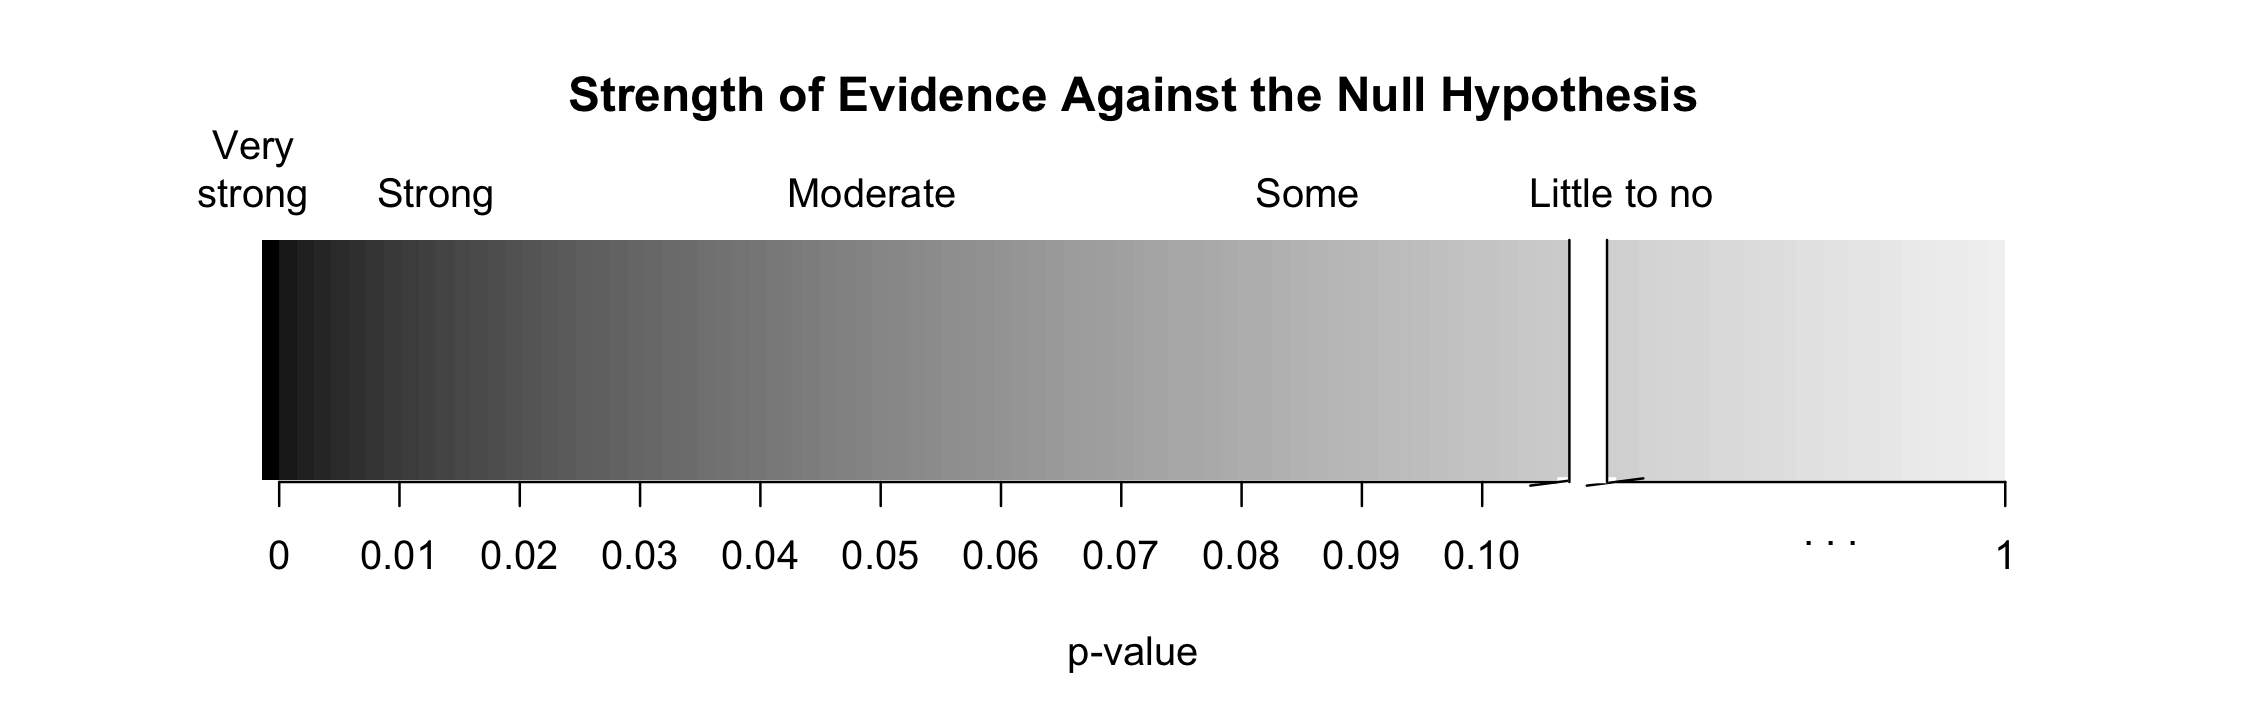
\includegraphics[width=0.9\linewidth]{images/soe_gradient_gray} \end{center}

\newpage

\begin{itemize}
\item
  \textbf{Conclusion} (to a hypothesis test): answers the research question. How much evidence is there in support of the alternative hypothesis?

  \begin{itemize}
  \item
    To write in context include:

    \begin{itemize}
    \item
      Amount of evidence
    \item
      Parameter of interest
    \item
      Direction of the alternative hypothesis
    \end{itemize}
  \end{itemize}
\item
  \textbf{Confidence interval}: an interval estimate for the parameter of interest; an interval of \emph{plausible values} for the parameter.

  \begin{itemize}
  \item
    A confidence interval helps us answer the following question about the population: How \emph{large} is the effect?
  \item
    To write in context include:

    \begin{itemize}
    \item
      How confident you are (e.g., 90\%, 95\%, 98\%, 99\%)
    \item
      Parameter of interest
    \item
      Calculated interval
    \end{itemize}
  \end{itemize}
\end{itemize}

\subsubsection{Simulation-based inference for a single proportion}\label{simulation-based-inference-for-a-single-proportion}

\begin{itemize}
\item
  \textbf{Conditions necessary to use simulation-based methods for inference for a single categorical variable}:

  \begin{itemize}
  \tightlist
  \item
    \textbf{Independence}: observational units must be independent of one another; the outcome of one observational unit should have no influence on the outcome of another.
  \end{itemize}
\item
  \textbf{Null distribution}: a sampling distribution of simulated sample statistics created under the assumption that the null hypothesis is true
\item
  \textbf{Simulation-based methods to create the null distribution}: a process of using a computer program (e.g., R) to simulate many samples that we would expect based on the null hypothesis.

  R code to use simulation methods for one categorical variable to find the p-value, \texttt{one\_proportion\_test} (from the \texttt{catstats} package), is shown below.

\begin{Shaded}
\begin{Highlighting}[]
\FunctionTok{one\_proportion\_test}\NormalTok{(}\AttributeTok{probability\_success =}\NormalTok{ xx, }\CommentTok{\# Null hypothesis value}
      \AttributeTok{sample\_size =}\NormalTok{ xx, }\CommentTok{\# Enter sample size}
      \AttributeTok{number\_repetitions =} \DecValTok{10000}\NormalTok{, }\CommentTok{\# Enter number of simulations}
      \AttributeTok{as\_extreme\_as =}\NormalTok{ xx, }\CommentTok{\# Observed statistic}
      \AttributeTok{direction =} \StringTok{"xx"}\NormalTok{, }\CommentTok{\# Specify direction of alternative hypothesis}
      \AttributeTok{summary\_measure =} \StringTok{"proportion"}\NormalTok{) }\CommentTok{\# Reporting proportion or number of successes?}
\end{Highlighting}
\end{Shaded}
\item
  \textbf{Bootstrapping}: creating a simulated sample of the same size as the original sample by sampling with replacement from the original sample.
\item
  \textbf{Simulation-based methods to create the bootstrap distribution}: a process of using a computer program to simulate many bootstrapped samples.

  R code to use simulation methods for one categorical variable to find a confidence interval, \texttt{one\_proportion\_bootstrap\_CI} (from the \texttt{catstats} package), is shown below.

\begin{Shaded}
\begin{Highlighting}[]
\FunctionTok{one\_proportion\_bootstrap\_CI}\NormalTok{(}\AttributeTok{sample\_size =}\NormalTok{ xx, }\CommentTok{\# Sample size}
                \AttributeTok{number\_successes =}\NormalTok{ xx, }\CommentTok{\# Observed number of successes}
                \AttributeTok{number\_repetitions =} \DecValTok{10000}\NormalTok{, }\CommentTok{\# Number of bootstrap samples to use}
                \AttributeTok{confidence\_level =} \FloatTok{0.95}\NormalTok{) }\CommentTok{\# Confidence level as a decimal}
\end{Highlighting}
\end{Shaded}
\item
  \textbf{Percentile method}: process to find the confidence interval from the bootstrap distribution.

  \begin{itemize}
  \item
    A 90\% confidence interval will be found between the 5th and 95th percentiles of the bootstrap distribution.
  \item
    A 95\% confidence interval will be found between the 2.5th and 97.5th percentiles of the bootstrap distribution.
  \item
    A 99\% confidence interval will be found between the 0.5th and 99.5th percentiles of the bootstrap distribution.
  \end{itemize}
\end{itemize}

\newpage

\section{Activity 4: Helper-Hinderer Part 1 --- Simulation-based Hypothesis Test}\label{activity-4-helper-hinderer-part-1-simulation-based-hypothesis-test}

\setstretch{1}

\subsection{Learning outcomes}\label{learning-outcomes-3}

\begin{itemize}
\item
  Identify the two possible explanations (one assuming the null hypothesis and one assuming the alternative hypothesis) for a relationship seen in sample data.
\item
  Given a research question involving a single categorical variable, construct the null and alternative hypotheses
  in words and using appropriate statistical symbols.
\item
  Describe and perform a simulation-based hypothesis test for a single proportion.
\end{itemize}

\subsection{Terminology review}\label{terminology-review-3}

In today's activity, we will work through a simulation-based hypothesis testing for a single categorical variable. Some terms covered in this activity are:

\begin{itemize}
\item
  Parameter of interest
\item
  Null hypothesis
\item
  Alternative hypothesis
\item
  Simulation
\end{itemize}

To review these concepts, see Chapters 9 \& 14 in your textbook.

\subsection{Steps of the statistical investigation process}\label{steps-of-the-statistical-investigation-process-1}

We will work through a five-step process to complete a hypothesis test for a single proportion, first introduced in the activity in week 1.

\begin{itemize}
\item
  \textbf{Ask a research question} that can be addressed by collecting data. What are the researchers trying to show?
\item
  \textbf{Design a study and collect data}. This step involves selecting the people or objects to be studied and how to gather relevant data on them.
\item
  \textbf{Summarize and visualize the data}. Calculate summary statistics and create graphical plots that best represent the research question.
\item
  \textbf{Use statistical analysis methods to draw inferences from the data}. Choose a statistical inference method appropriate for the data and identify the p-value and/or confidence interval after checking assumptions. In this study, we will focus on using randomization to generate a simulated p-value.
\item
  \textbf{Communicate the results and answer the research question}. Using the p-value and confidence interval from the analysis, determine whether the data provide statistical evidence against the null hypothesis. Write a conclusion that addresses the research question.
\end{itemize}

\newpage

\subsection*{Notes on Hypothesis Testing}\label{notes-on-hypothesis-testing}
\addcontentsline{toc}{subsection}{Notes on Hypothesis Testing}

\vspace{4in}

\subsection{Helper-Hinderer}\label{helper-hinderer}

A study by Hamblin, Wynn, and Bloom reported in Nature (Hamblin, Wynn, and Bloom 2007) was intended to check young kids' feelings about helpful and non-helpful behavior. Non-verbal infants ages 6 to 10 months were shown short videos with different shapes either helping or hindering the climber. As a class we will watch this short video to see how the experiment was run: \url{https://youtu.be/anCaGBsBOxM}. Researchers were hoping to assess: Are infants more likely to choose the helper toy? In the study, of the 16 infants age 6 to 10 months, 14 chose the \emph{helper} toy and 2 chose the \emph{hinderer} toy.

\begin{itemize}
\item
  Observational units:
\item
  Variable:
\item
  Type of variable:
\item
  Success:
\end{itemize}

\subsubsection*{Ask a research question}\label{ask-a-research-question}
\addcontentsline{toc}{subsubsection}{Ask a research question}

\begin{itemize}
\tightlist
\item
  Research question:
\end{itemize}

\vspace{0.2in}

\subsubsection*{Design a study and collect data}\label{design-a-study-and-collect-data}
\addcontentsline{toc}{subsubsection}{Design a study and collect data}

Before using statistical inference methods, we must check that the cases are independent. The sample observations are independent if the outcome of one observation does not influence the outcome of another. One way this condition is met is if data come from a simple random sample of the target population.

\begin{enumerate}
\def\labelenumi{\arabic{enumi}.}
\tightlist
\item
  Are the cases independent? Justify your answer.
\end{enumerate}

\vspace{0.8in}

\subsubsection*{R code}\label{r-code}
\addcontentsline{toc}{subsubsection}{R code}

For almost all activities and labs it will be necessary to upload the provided R script file from D2L for that day. Your instructor will highlight a few steps in uploading files to and using RStudio.

The following are the steps to upload the necessary R script file for this activity:

\begin{itemize}
\item
  Download the Activity R script file from D2L.
\item
  Click ``Upload'' in the ``Files'' tab in the bottom right window of RStudio. In the pop-up window, click ``Choose File'', and navigate to the folder where the Activity R script file is saved (most likely in your downloads folder). Click ``Open''; then click ``Ok''.
\item
  You should see the uploaded file appear in the list of files in the bottom right window. Click on the file name to open the file in the Editor window (upper left window).
\end{itemize}

Notice that the first threelines of code contain a prompt called \texttt{library}. Packages needed to run functions in R are stored in directories called libraries. When using the MSU RStudio server, all the packages needed for the class are already installed. We simply must tell R which packages we need for each R script file. We use the prompt \texttt{library} to load each \textbf{package} (or library) needed for each activity. Note, these \texttt{library} lines MUST be run each time you open a R script file in order for the functions in R to work.

\begin{itemize}
\tightlist
\item
  Highlight and run lines 1--3 to load the packages needed for this activity. Notice the use of the \# symbol in the R script file. This symbol is not part of the R code. It is used by these authors to add comments to the R code and explain what each call is telling the program to do.
\end{itemize}

R will ignore everything after a \# symbol when executing the code. Refer to the instructions following the \# symbol to understand what you need to enter in the code.

\begin{Shaded}
\begin{Highlighting}[]
\FunctionTok{library}\NormalTok{(tidyverse)}
\FunctionTok{library}\NormalTok{(ggplot2)}
\FunctionTok{library}\NormalTok{(catstats)}
\end{Highlighting}
\end{Shaded}

Throughout activities, we will often include the R code you would use in order to produce output or plots. These ``code chunks'' appear in gray. In the code chunk below, we demonstrate how to read the data set into R using the \texttt{read.csv()} function. The line of code shown below (line 7 in the R script file) reads in the data set and names the data set \texttt{infants}.

\subsubsection*{Summarize and visualize the data}\label{summarize-and-visualize-the-data}
\addcontentsline{toc}{subsubsection}{Summarize and visualize the data}

The following code reads in the data set and gives the number of infants in each level of the variable, whether the infant chose the helper or the hinderer.

\begin{itemize}
\tightlist
\item
  Highlight and run lines 7 and 8 to check that you get the same counts as shown below
\end{itemize}

\begin{Shaded}
\begin{Highlighting}[]
 \CommentTok{\# Read in data set}
\NormalTok{infants }\OtherTok{\textless{}{-}} \FunctionTok{read.csv}\NormalTok{(}\StringTok{"https://math.montana.edu/courses/s216/data/infantchoice.csv"}\NormalTok{)}
\NormalTok{infants }\SpecialCharTok{\%\textgreater{}\%} \FunctionTok{count}\NormalTok{(choice)  }\CommentTok{\# Count number in each choice category}
\end{Highlighting}
\end{Shaded}

\begin{verbatim}
#>     choice  n
#> 1   helper 14
#> 2 hinderer  2
\end{verbatim}

The following formula is used to calculate the proportion of successes in the sample.

\[\hat{p} = \frac{\mbox{number of successes}}{\mbox{total number of observational units}}\]
\newpage

\begin{enumerate}
\def\labelenumi{\arabic{enumi}.}
\setcounter{enumi}{1}
\tightlist
\item
  Using the R output and the formula given, calculate the summary statistic (sample proportion) to represent the research question. Recall that \texttt{choosing\ the\ helper\ toy} is a considered a success. Use appropriate notation.
\end{enumerate}

\vspace{0.5in}

To visually display this data we can use either a frequency bar plot or a relative frequency bar plot.

\begin{itemize}
\item
  Enter the variable name \texttt{choice} for \texttt{variable} in the R code to create the frequency bar plot.
\item
  Note the name of the title is given in line 16 and includes the \textbf{type of plot}, \textbf{observational units}, and \textbf{variable name}.
\item
  Highlight and run lines 13--19 to create the plot
\end{itemize}

\begin{Shaded}
\begin{Highlighting}[]
\NormalTok{infants }\SpecialCharTok{\%\textgreater{}\%} \CommentTok{\# Data set piped into...}
    \FunctionTok{ggplot}\NormalTok{(}\FunctionTok{aes}\NormalTok{(}\AttributeTok{x =}\NormalTok{ variable)) }\SpecialCharTok{+}   \CommentTok{\# This specifies the variable}
    \FunctionTok{geom\_bar}\NormalTok{(}\AttributeTok{stat =} \StringTok{"count"}\NormalTok{) }\SpecialCharTok{+}  \CommentTok{\# Tell it to make a bar plot}
    \FunctionTok{labs}\NormalTok{(}\AttributeTok{title =} \StringTok{"Frequency Bar Plot of Toy Choice for Pre{-}verbal Infants"}\NormalTok{,  }
       \CommentTok{\# Give your plot a title}
       \AttributeTok{x =} \StringTok{"Toy Choice"}\NormalTok{,   }\CommentTok{\# Label the x axis}
       \AttributeTok{y =} \StringTok{"Frequency"}\NormalTok{)  }\CommentTok{\# Label the y axis}
\end{Highlighting}
\end{Shaded}

\begin{enumerate}
\def\labelenumi{\arabic{enumi}.}
\setcounter{enumi}{2}
\tightlist
\item
  Sketch the frequency bar plot created below.
\end{enumerate}

\vspace{1.8in}

We could also choose to display the data as a proportion in a \textbf{relative frequency} bar plot. To find the relative frequency, the count in each level of \texttt{choice} is divided by the sample size. This calculation is the sample proportion for each level of \texttt{choice}. Notice that in the following code we told R to create a bar plot with proportions.

\begin{itemize}
\tightlist
\item
  In the R script file, highlight and run lines 23--29 to create the relative frequency bar plot.
\end{itemize}

\begin{Shaded}
\begin{Highlighting}[]
\NormalTok{infants }\SpecialCharTok{\%\textgreater{}\%} \CommentTok{\# Data set piped into...}
    \FunctionTok{ggplot}\NormalTok{(}\FunctionTok{aes}\NormalTok{(}\AttributeTok{x =}\NormalTok{ choice)) }\SpecialCharTok{+}   \CommentTok{\# This specifies the variable}
    \FunctionTok{geom\_bar}\NormalTok{(}\FunctionTok{aes}\NormalTok{(}\AttributeTok{y =} \FunctionTok{after\_stat}\NormalTok{(prop), }\AttributeTok{group =} \DecValTok{1}\NormalTok{)) }\SpecialCharTok{+}  \CommentTok{\# Tell it to make a bar plot with proportions}
    \FunctionTok{labs}\NormalTok{(}\AttributeTok{title =} \StringTok{"Relative Frequency Bar Plot of Toy Choice for Pre{-}verbal Infants"}\NormalTok{,  }
       \CommentTok{\# Give your plot a title}
       \AttributeTok{x =} \StringTok{"Toy Choice"}\NormalTok{,   }\CommentTok{\# Label the x axis}
       \AttributeTok{y =} \StringTok{"Relative Frequency"}\NormalTok{)  }\CommentTok{\# Label the y axis}
\end{Highlighting}
\end{Shaded}

\begin{center}\includegraphics[width=0.5\linewidth]{03-A04-inference-1cat_test-simulation_files/figure-latex/unnamed-chunk-4-1} \end{center}

\begin{enumerate}
\def\labelenumi{\arabic{enumi}.}
\setcounter{enumi}{3}
\tightlist
\item
  Which features in the relative frequency bar plot are the same as the frequency bar plot? Which are different?
\end{enumerate}

\vspace{0.5in}

We cannot assess whether infants are more likely to choose the helper toy based on the statistic and plot alone. The next step is to analyze the data by using a hypothesis test to discover if there is evidence against the null hypothesis.

\subsubsection*{Use statistical analysis methods to draw inferences from the data}\label{use-statistical-analysis-methods-to-draw-inferences-from-the-data}
\addcontentsline{toc}{subsubsection}{Use statistical analysis methods to draw inferences from the data}

When performing a hypothesis test, we must first identify the null hypothesis. The null hypothesis is written about the parameter of interest, or the value that summarizes the variable in the population.

The parameter of interest is a statement about what we want to find about the population. The following must be included when writing the parameter of interest.

\begin{itemize}
\item
  Population word (true, long-run, population)
\item
  Summary measure (depends on the type of data)
\item
  Context

  \begin{itemize}
  \item
    Observational units
  \item
    Variable(s)
  \end{itemize}
\end{itemize}

\textbf{Parameter of interest:}

\vspace{0.5in}

If the children are just randomly choosing the toy, we would expect half (0.5) of the infants to choose the helper toy. This is the null value for our study.

\textbf{Null Hypothesis (in words):}

\vspace{0.5in}

The notation used for a population proportion (or probability, or true proportion) is \(\pi\). Since this summarizes a population, it is a parameter. When writing the \textbf{null hypothesis} in notation, we set the parameter equal to the null value, \(H_0: \pi = \pi_0\).

\textbf{Null Hypothesis (in notation):}

\vspace{0.5in}

The \textbf{alternative hypothesis} is the claim to be tested and the direction of the claim (less than, greater than, or not equal to) is based on the research question.

\begin{itemize}
\tightlist
\item
  Based on the research question from question 1, are we testing that the parameter is greater than 0.5, less than 0.5 or different than 0.5?
\end{itemize}

\vspace{0.2in}

\textbf{Alternative hypothesis (in words):}

\vspace{0.5in}

\textbf{Alternative hypothesis (in notation):}

\vspace{0.5in}

Remember that when utilizing a hypothesis test, we are evaluating two competing possibilities. For this study the \textbf{two possibilities} are either\ldots{}

\begin{itemize}
\item
  The true proportion of infants who choose the helper is 0.5 and our results just occurred by random chance; or,
\item
  The true proportion of infants who choose the helper is greater than 0.5 and our results reflect this.
\end{itemize}

Notice that these two competing possibilities represent the null and alternative hypotheses.

We will now simulate one sample of a \textbf{null distribution} of sample proportions. The null distribution is created under the assumption the null hypothesis is true. In this case, we assume the true proportion of infants who choose the helper is 0.5, so we will create 10000 (or more) different simulations of 16 infants under this assumption.

Let's think about how to use a coin to create one simulation of 16 infants under the assumption the null hypothesis is true. Let heads equal infant chose the helper toy and tails equal infant chose the hinderer toy.

\begin{enumerate}
\def\labelenumi{\arabic{enumi}.}
\setcounter{enumi}{4}
\tightlist
\item
  How many times would you flip a coin to simulate the sample of infants?
\end{enumerate}

\vspace{0.2in}

\begin{enumerate}
\def\labelenumi{\arabic{enumi}.}
\setcounter{enumi}{5}
\tightlist
\item
  Flip a coin 16 times recording the number of times the coin lands on heads. This represents one simulated sample of 16 infants randomly choosing the toy. Calculate the proportion of coin flips that resulted in heads.
\end{enumerate}

\vspace{0.2in}

\begin{enumerate}
\def\labelenumi{\arabic{enumi}.}
\setcounter{enumi}{6}
\tightlist
\item
  Is the value from question 6 closer to 0.5, the null value, or closer to the sample proportion, 0.875?
\end{enumerate}

\vspace{0.2in}

Report the number of coin flips you got as indicated by your instructor.

\begin{enumerate}
\def\labelenumi{\arabic{enumi}.}
\setcounter{enumi}{7}
\tightlist
\item
  Sketch the graph created by your instructor of each student's proportion of heads out of 16 coin flips.
\end{enumerate}

\vspace{2in}

\begin{enumerate}
\def\labelenumi{\arabic{enumi}.}
\setcounter{enumi}{8}
\tightlist
\item
  Circle the observed statistic (value from question 2) on the distribution shown above. Where does this statistic fall in this distribution: Is it near the center of the distribution (near 0.5) or in one of the tails of the distribution?
\end{enumerate}

\vspace{0.2in}

\begin{enumerate}
\def\labelenumi{\arabic{enumi}.}
\setcounter{enumi}{9}
\tightlist
\item
  Is the observed statistic likely to happen or unlikely to happen if the true proportion of infants who choose the helper is 0.5? Explain your answer using the plot.
\end{enumerate}

\vspace{0.8in}

In the next class, we will continue to assess the strength of evidence against the null hypothesis by using a computer to simulate 10000 samples when we assume the null hypothesis is true.

\subsection{Take-home messages}\label{take-home-messages-3}

\begin{enumerate}
\def\labelenumi{\arabic{enumi}.}
\item
  Two types of plots are used for plotting categorical variables: frequency bar plots, relative frequency bar plots.
\item
  In a hypothesis test we have two competing hypotheses, the null hypothesis and the alternative hypothesis. The null hypothesis represents either a skeptical perspective or a perspective of no difference or no effect. The alternative hypothesis represents a new perspective such as the possibility that there has been a change or that there is a treatment effect in an experiment.
\item
  In a simulation-based test, we create a distribution of possible simulated statistics for our sample if the null hypothesis is true. Then we see if the calculated observed statistic from the data is likely or unlikely to occur when compared to the null distribution.
\item
  To create one simulated sample on the null distribution for a sample proportion, spin a spinner with probability equal to \(\pi_0\) (the null value), \(n\) times or draw with replacement \(n\) times from a deck of cards created to reflect \(\pi_0\) as the probability of success. Calculate and plot the proportion of successes from the simulated sample.
\end{enumerate}

\subsection{Additional notes}\label{additional-notes-3}

Use this space to summarize your thoughts and take additional notes on today's activity and material covered.

\newpage

\section{Activity 5: Helper-Hinderer (continued)}\label{activity-5-helper-hinderer-continued}

\setstretch{1}

\subsection{Learning outcomes}\label{learning-outcomes-4}

\begin{itemize}
\item
  Describe and perform a simulation-based hypothesis test for a single proportion.
\item
  Interpret and evaluate a p-value for a simulation-based hypothesis test for a single proportion.
\item
  Explore what a p-value represents
\end{itemize}

\subsection{Steps of the statistical investigation process}\label{steps-of-the-statistical-investigation-process-2}

In today's activity we will continue with steps 4 and 5 in the statistical investigation process. We will continue to assess the Helper-Hinderer study from last class.

\begin{itemize}
\item
  \textbf{Ask a research question} that can be addressed by collecting data. What are the researchers trying to show?
\item
  \textbf{Design a study and collect data}. This step involves selecting the people or objects to be studied and how to gather relevant data on them.
\item
  \textbf{Summarize and visualize the data}. Calculate summary statistics and create graphical plots that best represent the research question.
\item
  \textbf{Use statistical analysis methods to draw inferences from the data}. Choose a statistical inference method appropriate for the data and identify the p-value and/or confidence interval after checking assumptions. In this study, we will focus on using randomization to generate a simulated p-value.
\item
  \textbf{Communicate the results and answer the research question}. Using the p-value and confidence interval from the analysis, determine whether the data provide statistical evidence against the null hypothesis. Write a conclusion that addresses the research question.
\end{itemize}

\subsection{Helper-Hinderer}\label{helper-hinderer-1}

In class today, we will revisit the study on infants as described below.

A study by Hamblin, Wynn, and Bloom reported in Nature (Hamblin, Wynn, and Bloom 2007) was intended to check young kids' feelings about helpful and non-helpful behavior. Non-verbal infants ages 6 to 10 months were shown short videos with different shapes either helping or hindering the climber. As a class we will watch this short video to see how the experiment was run: \url{https://youtu.be/anCaGBsBOxM}. Researchers were hoping to assess: Are infants more likely to choose the helper toy? In the study, of the 16 infants age 6 to 10 months, 14 chose the \emph{helper} toy and 2 chose the \emph{hinderer} toy.

\begin{enumerate}
\def\labelenumi{\arabic{enumi}.}
\tightlist
\item
  Report the sample proportion (summary statistic) calculated in the previous activity.
\end{enumerate}

\vspace{0.3in}

\begin{enumerate}
\def\labelenumi{\arabic{enumi}.}
\setcounter{enumi}{1}
\tightlist
\item
  Write the alternative hypothesis in words in context of the problem. Remember the direction we are testing is dependent on the research question.
\end{enumerate}

\vspace{0.8in}

Today, we will use the computer to simulate a null distribution of 10000 different samples of 16 infants, plotting the proportion who chose the helper in each sample, based on the assumption that the true proportion of infants who choose the helper is 0.5 (or that the null hypothesis is true).

\newpage

To use the computer simulation, we will need to enter the

\begin{itemize}
\tightlist
\item
  assumed ``probability of success'' (\(\pi_0\)),
\item
  ``sample size'' (the number of observational units or cases in the sample),
\item
  ``number of repetitions'' (the number of samples to be generated - typically we use 10000),
\item
  ``as extreme as'' (the observed statistic), and
\item
  the ``direction'' (matches the direction of the alternative hypothesis).
\end{itemize}

\begin{enumerate}
\def\labelenumi{\arabic{enumi}.}
\setcounter{enumi}{2}
\tightlist
\item
  What values should be entered for each of the following into the one proportion test to create 10000 simulations?
\end{enumerate}

\vspace{1mm}

\begin{itemize}
\tightlist
\item
  Probability of success (null value):
\end{itemize}

\vspace{.2in}

\begin{itemize}
\tightlist
\item
  Sample size (n):
\end{itemize}

\vspace{.2in}

\begin{itemize}
\tightlist
\item
  Number of repetitions (always use 10000 simulations):
\end{itemize}

\vspace{.2in}

\begin{itemize}
\tightlist
\item
  As extreme as (value of statistic):
\end{itemize}

\vspace{.2in}

\begin{itemize}
\tightlist
\item
  Direction (\texttt{"greater"}, \texttt{"less"}, or \texttt{"two-sided"}):
\end{itemize}

We will use the \texttt{one\_proportion\_test()} function in \texttt{R} (in the \texttt{catstats} package) to simulate the null distribution of sample proportions and compute a p-value. Using the provided \texttt{R} script file, fill in the values/words for each \texttt{xx} with your answers from question 3 in the one proportion test to create a null distribution with 10000 simulations. Then highlight and run lines 1--16.

\begin{Shaded}
\begin{Highlighting}[]
\FunctionTok{one\_proportion\_test}\NormalTok{(}\AttributeTok{probability\_success =}\NormalTok{ xx, }\CommentTok{\# Null hypothesis value}
          \AttributeTok{sample\_size =}\NormalTok{ xx, }\CommentTok{\# Enter sample size}
          \AttributeTok{number\_repetitions =} \DecValTok{10000}\NormalTok{, }\CommentTok{\# Enter number of simulations}
          \AttributeTok{as\_extreme\_as =}\NormalTok{ xx, }\CommentTok{\# Observed statistic}
          \AttributeTok{direction =} \StringTok{"xx"}\NormalTok{, }\CommentTok{\# Specify direction of alternative hypothesis}
          \AttributeTok{summary\_measure =} \StringTok{"proportion"}\NormalTok{) }\CommentTok{\# Reporting proportion or number of successes?}
\end{Highlighting}
\end{Shaded}

\begin{enumerate}
\def\labelenumi{\arabic{enumi}.}
\setcounter{enumi}{3}
\tightlist
\item
  Sketch the null distribution created from the \texttt{R} code here.
\end{enumerate}

\vspace{1.8in}

\subsection*{Notes on the null distribution}\label{notes-on-the-null-distribution}
\addcontentsline{toc}{subsection}{Notes on the null distribution}

\vspace{2in}

\begin{enumerate}
\def\labelenumi{\arabic{enumi}.}
\setcounter{enumi}{4}
\tightlist
\item
  Circle the observed statistic (value from question 1) on the distribution you drew in question 4. Where does this statistic fall in the null distribution: Is it near the center of the distribution (near 0.5) or in one of the tails of the distribution?
\end{enumerate}

\vspace{0.3in}

\begin{enumerate}
\def\labelenumi{\arabic{enumi}.}
\setcounter{enumi}{5}
\tightlist
\item
  Is the observed statistic likely to happen or unlikely to happen if the true proportion of infants who choose the helper is 0.5? Explain your answer using the plot.
\end{enumerate}

\vspace{0.5in}

\begin{enumerate}
\def\labelenumi{\arabic{enumi}.}
\setcounter{enumi}{6}
\tightlist
\item
  Using the simulation, what is the proportion of simulated samples that generated a sample proportion at the observed statistic or greater, if the true proportion of infants who choose the helper is 0.5? \emph{Hint}: Look under the simulation.
\end{enumerate}

\vspace{0.3in}

\subsection*{Notes on the p-value}\label{notes-on-the-p-value}
\addcontentsline{toc}{subsection}{Notes on the p-value}

The value in question 7 is the \textbf{p-value}. The smaller the p-value, the more evidence we have against the null hypothesis.

\vspace{1.5in}

\begin{center}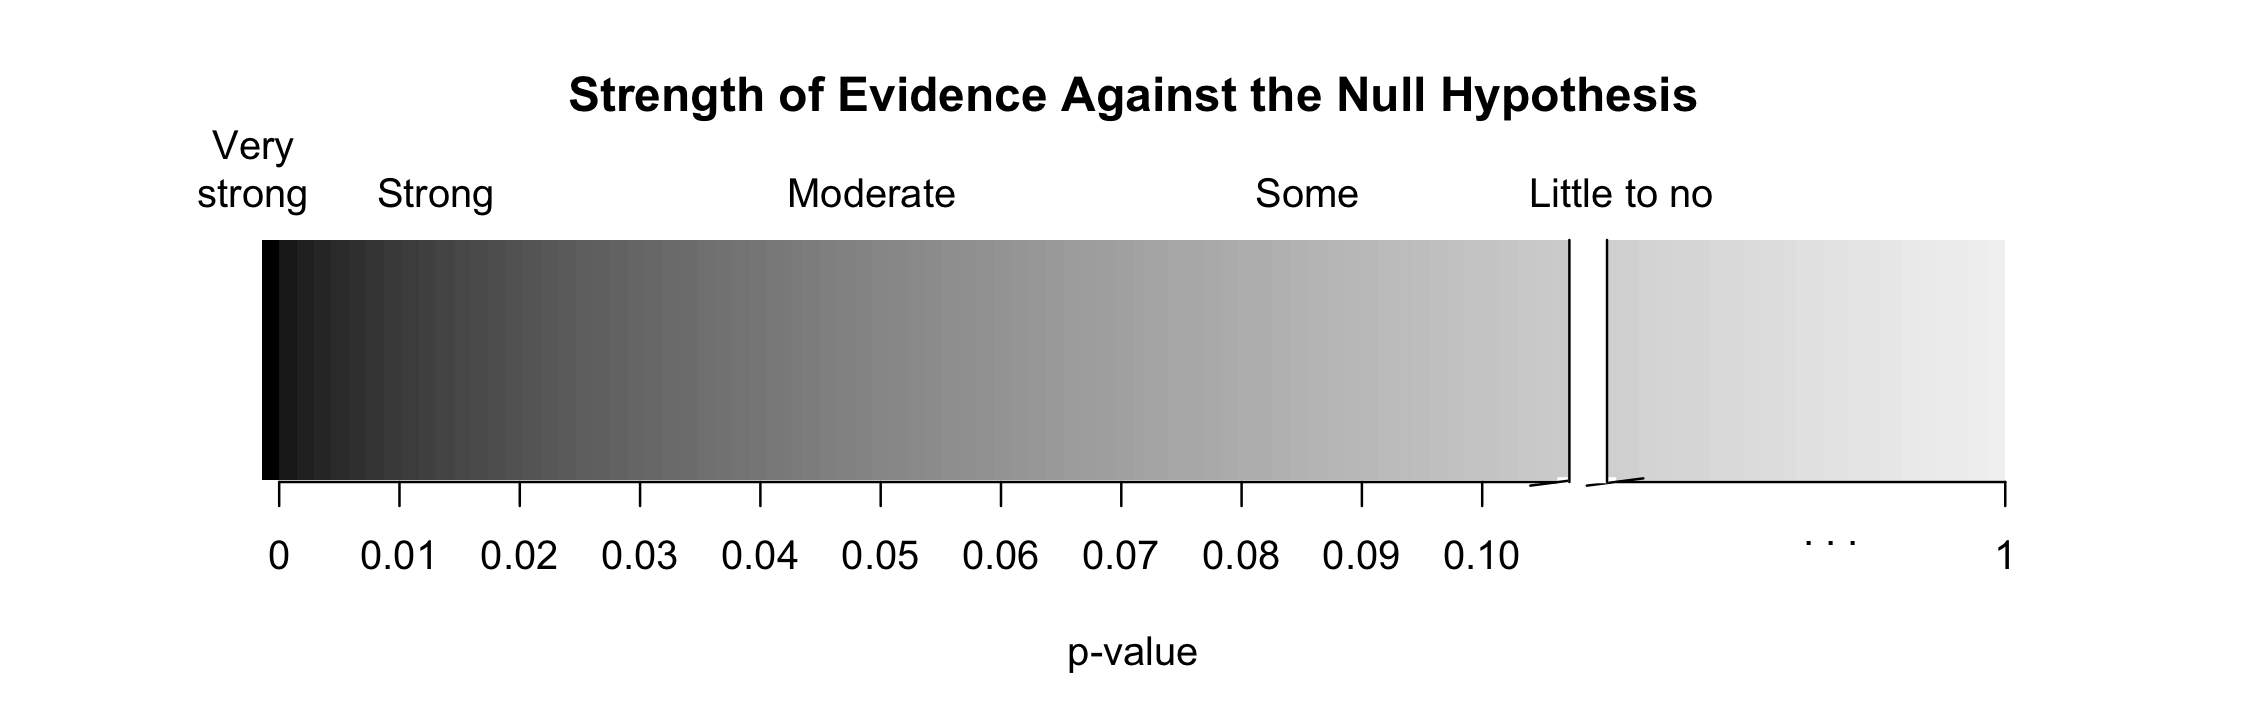
\includegraphics[width=0.9\linewidth]{images/soe_gradient_gray} \end{center}

\subsubsection*{Interpret the p-value}\label{interpret-the-p-value}
\addcontentsline{toc}{subsubsection}{Interpret the p-value}

The p-value measures the probability that we observe a sample proportion as extreme as what was seen in the data or more extreme (matching the direction of the Ha) IF the null hypothesis is true. This is a conditional probability, calculated dependent on the null hypothesis being true. Represented in probability notation:

\[P(\text{statistic or more extreme|the null hypothesis is true})\]

\textbf{p-value interpretation:}

\vspace{1in}

\subsubsection*{Communicate the results and answer the research question}\label{communicate-the-results-and-answer-the-research-question}
\addcontentsline{toc}{subsubsection}{Communicate the results and answer the research question}

When we write a conclusion we answer the research question by stating how much evidence there is for the alternative hypothesis.

\textbf{Conclusion:}

\vspace{1in}

\subsubsection*{Generalization}\label{generalization}
\addcontentsline{toc}{subsubsection}{Generalization}

\begin{enumerate}
\def\labelenumi{\arabic{enumi}.}
\setcounter{enumi}{7}
\tightlist
\item
  To what group of observational units can the results be generalized to?
\end{enumerate}

\vspace{0.5in}

\subsection{Take-home messages}\label{take-home-messages-4}

\begin{enumerate}
\def\labelenumi{\arabic{enumi}.}
\item
  The null distribution is created based on the assumption the null hypothesis is true. We compare the sample statistic to the distribution to find the likelihood of observing this statistic.
\item
  The p-value measures the probability of observing the sample statistic or more extreme (in direction of the alternative hypothesis) is the null hypothesis is true.
\item
  The smaller the p-value of the test, the more evidence there is \textbf{against} the null hypothesis.
\end{enumerate}

\subsection{Additional notes}\label{additional-notes-4}

Use this space to summarize your thoughts and take additional notes on today's activity and material covered.

\newpage

\section{Activity 6: Helper-Hinderer --- Simulation-based Confidence Interval}\label{activity-6-helper-hinderer-simulation-based-confidence-interval}

\setstretch{1}

\subsection{Learning outcomes}\label{learning-outcomes-5}

\begin{itemize}
\item
  Use bootstrapping to find a confidence interval for a single proportion.
\item
  Interpret a confidence interval for a single proportion.
\end{itemize}

\subsection{Terminology review}\label{terminology-review-4}

In today's activity, we will introduce simulation-based confidence intervals for a single proportion. Some terms covered in this activity are:

\begin{itemize}
\item
  Parameter of interest
\item
  Bootstrapping
\item
  Confidence interval
\end{itemize}

To review these concepts, see Chapters 10 \& 14 in your textbook.

\subsection{Helper-Hinderer}\label{helper-hinderer-2}

In the last class, we found very strong evidence that the true proportion of infants who will choose the helper character is greater than 0.5. But what \emph{is} the true proportion of infants who will choose the helper character? We will use this same study to estimate this parameter of interest by creating a confidence interval.

As a reminder: A study by Hamblin, Wynn, and Bloom reported in Nature (Hamblin, Wynn, and Bloom 2007) was intended to check young kids' feelings about helpful and non-helpful behavior. Non-verbal infants ages 6 to 10 months were shown short videos with different shapes either helping or hindering the climber. Researchers were hoping to assess: Are infants more likely to preferentially choose the helper toy? In the study, of the 16 infants age 6 to 10 months, 14 chose the \emph{helper} toy and 2 chose the \emph{hinderer} toy.

A \textbf{point estimate} (our observed statistic) provides a single plausible value for a parameter. However, a point estimate is rarely perfect; usually there is some error in the estimate. In addition to supplying a point estimate of a parameter, a next logical step would be to provide a plausible \emph{range} of values for the parameter. This plausible range of values for the population parameter is called an \textbf{interval estimate} or \textbf{confidence interval}.

\subsubsection*{Activity intro}\label{activity-intro}
\addcontentsline{toc}{subsubsection}{Activity intro}

\begin{enumerate}
\def\labelenumi{\arabic{enumi}.}
\tightlist
\item
  What is the value of the point estimate (sample statistic)?
\end{enumerate}

\vspace{0.3in}

\begin{enumerate}
\def\labelenumi{\arabic{enumi}.}
\setcounter{enumi}{1}
\tightlist
\item
  If we took another random sample of 16 infants, would we get the exact same point estimate? Explain why or why not.
\end{enumerate}

\vspace{0.5in}

In today's activity, we will use bootstrapping to find a 95\% confidence interval for \(\pi\), the parameter of interest.

\subsection*{Notes on Confidence Intervals}\label{notes-on-confidence-intervals}
\addcontentsline{toc}{subsection}{Notes on Confidence Intervals}

\vspace{2in}

\subsubsection*{Use statistical analysis methods to draw inferences from the data}\label{use-statistical-analysis-methods-to-draw-inferences-from-the-data-1}
\addcontentsline{toc}{subsubsection}{Use statistical analysis methods to draw inferences from the data}

\begin{enumerate}
\def\labelenumi{\arabic{enumi}.}
\setcounter{enumi}{2}
\tightlist
\item
  Write out the parameter of interest in words, in context of the study. What does \(\pi\) represent?
\end{enumerate}

\vspace{0.5in}

To create the null distribution we flipped a coin 16 times to simulate infants randomly choosing the helper toy with a probability of 50\%.

\begin{enumerate}
\def\labelenumi{\arabic{enumi}.}
\setcounter{enumi}{3}
\tightlist
\item
  Why can't we use a coin to simulate the bootstrap distribution.
\end{enumerate}

\vspace{0.7in}

To create the bootstrap distribution.

\begin{itemize}
\item
  First we would label the cards to represent the sample statistic: 14 helper and 2 hinderer.
\item
  Sample with replacement 16 times
\end{itemize}

\begin{enumerate}
\def\labelenumi{\arabic{enumi}.}
\setcounter{enumi}{4}
\tightlist
\item
  Using the cards provided by your instructor, create one bootstrap sample. Report your simulated sample proportion on the whiteboard.
\end{enumerate}

\vspace{0.3in}

To use the computer simulation to create a bootstrap distribution, we will need to enter the

\begin{itemize}
\tightlist
\item
  ``sample size'' (the number of observational units or cases in the sample),
\item
  ``number of successes'' (the number of cases that choose the helper character),
\item
  ``number of repetitions'' (the number of samples to be generated), and
\item
  the ``confidence level'' (which level of confidence are we using to create the confidence interval).
\end{itemize}

\begin{enumerate}
\def\labelenumi{\arabic{enumi}.}
\setcounter{enumi}{5}
\tightlist
\item
  What values should be entered for each of the following into the simulation to create the bootstrap distribution of sample proportions to find a 95\% confidence interval?
  \vspace{1mm}
\end{enumerate}

\begin{itemize}
\tightlist
\item
  Sample size (n):
\end{itemize}

\vspace{.1in}

\begin{itemize}
\tightlist
\item
  Number of successes:
\end{itemize}

\vspace{.1in}

\begin{itemize}
\tightlist
\item
  Number of repetitions (at least 10000):
\end{itemize}

\vspace{.1in}

\begin{itemize}
\tightlist
\item
  Confidence level (as a decimal):
\end{itemize}

\vspace{.1in}

We will use the \texttt{one\_proportion\_bootstrap\_CI()} function in R (in the \texttt{catstats} package) to simulate the bootstrap distribution of sample proportions and calculate a confidence interval. Using the provided R script file, fill in the values/words for each \texttt{xx} with your answers from question 6 in the one proportion bootstrap confidence interval (CI) code to create a bootstrap distribution with 10000 simulations. Then highlight and run lines 1--9.

\begin{Shaded}
\begin{Highlighting}[]
\FunctionTok{one\_proportion\_bootstrap\_CI}\NormalTok{(}\AttributeTok{sample\_size =}\NormalTok{ xx, }\CommentTok{\# Sample size}
                    \AttributeTok{number\_successes =}\NormalTok{ xx, }\CommentTok{\# Observed number of successes}
                    \AttributeTok{number\_repetitions =} \DecValTok{10000}\NormalTok{, }\CommentTok{\# Number of bootstrap samples to use}
                    \AttributeTok{confidence\_level =}\NormalTok{ xx) }\CommentTok{\# Confidence level as a decimal}
\end{Highlighting}
\end{Shaded}

\begin{enumerate}
\def\labelenumi{\arabic{enumi}.}
\setcounter{enumi}{6}
\tightlist
\item
  Sketch the bootstrap distribution created below.
\end{enumerate}

\vspace{1.8in}

\subsection*{Notes on the bootstrap distribution}\label{notes-on-the-bootstrap-distribution}
\addcontentsline{toc}{subsection}{Notes on the bootstrap distribution}

\vspace{1.5in}

\textbf{95\% Confidence Interval:}

\textbf{Interpretation of the 95\% confidence interval in context.}

\vspace{.6in}

\subsubsection*{Communicate the results and answer the research question}\label{communicate-the-results-and-answer-the-research-question-1}
\addcontentsline{toc}{subsubsection}{Communicate the results and answer the research question}

\begin{enumerate}
\def\labelenumi{\arabic{enumi}.}
\setcounter{enumi}{7}
\tightlist
\item
  Is the value 0.5 (the null value) in the 95\% confidence interval?
\end{enumerate}

\vspace{.2in}

~~~Explain how this indicates that the p-value provides strong evidence against the null.

\vspace{0.5in}

\subsubsection*{Effect of confidence level}\label{effect-of-confidence-level}
\addcontentsline{toc}{subsubsection}{Effect of confidence level}

\begin{enumerate}
\def\labelenumi{\arabic{enumi}.}
\setcounter{enumi}{8}
\tightlist
\item
  Suppose instead of finding a 95\% confidence interval, we found a 90\% confidence interval. Would you expect the 90\% confidence interval to be narrower or wider? Explain your answer.
\end{enumerate}

\vspace{0.4in}

\begin{enumerate}
\def\labelenumi{\arabic{enumi}.}
\setcounter{enumi}{9}
\tightlist
\item
  The following R code produced the bootstrap distribution with 10000 simulations that follows. Circle the value that changed in the code.
\end{enumerate}

\begin{Shaded}
\begin{Highlighting}[]
\FunctionTok{one\_proportion\_bootstrap\_CI}\NormalTok{(}\AttributeTok{sample\_size =} \DecValTok{16}\NormalTok{, }\CommentTok{\# Sample size}
                    \AttributeTok{number\_successes =} \DecValTok{14}\NormalTok{, }\CommentTok{\# Observed number of successes}
                    \AttributeTok{number\_repetitions =} \DecValTok{10000}\NormalTok{, }\CommentTok{\# Number of bootstrap samples to use}
                    \AttributeTok{confidence\_level =} \FloatTok{0.90}\NormalTok{) }\CommentTok{\# Confidence level as a decimal}
\end{Highlighting}
\end{Shaded}

\begin{center}\includegraphics[width=0.7\linewidth]{03-A06-inference-1cat_CI-simulation_files/figure-latex/unnamed-chunk-2-1} \end{center}

\begin{enumerate}
\def\labelenumi{\arabic{enumi}.}
\setcounter{enumi}{10}
\tightlist
\item
  Report both the 95\% confidence interval and the 90\% confidence interval (question 10). Is the 90\% confidence interval narrower or wider than the 95\% confidence interval?
\end{enumerate}

\vspace{0.5in}

\setstretch{1.5}

\subsubsection*{Concluding paragraph}\label{concluding-paragraph}
\addcontentsline{toc}{subsubsection}{Concluding paragraph}

In many of our studies we will write a paragraph summarizing the results of the study.

Researchers were interested if infants observe social cues and would be more likely to choose the helper toy. In a sample of \_\_\_\_\_\_\_\_\_\_\_\_\_infants, \_\_\_\_\_\_\_\_\_\_\_\_\_\_\_chose the helper toy. A simulation null distribution with 10000 simulations was created in RStudio. The p-value was found by calculating the proportion of simulations in the null distribution at the sample statistic of 0.875 and greater. This resulted in a p-value of \_\_\_\_\_\_\_\_\_\_\_\_\_\_\_. We would observe a sample proportion of \_\_\_\_\_\_\_\_\_\_\_\_\_\_\_\_\_\_\_\_\_\_ or \_\_\_\_\_\_\_\_\_\_\_\_\_\_\_\_\_\_\_\_\_ with a probability of \_\_\_\_\_\_\_\_\_\_\_\_\_\_\_\_\_\_\_\\
IF we assume \_\_\_\_\_\_\_\_\_\_\_\_\_\_\_\_\_\_\_\_\_\_\_\_\_\_\_\_\_\_\_\_\_\_\_\_\_\_\_\_\_\_\_\_\_\_\_.
Based on this p-value, there is \_\_\_\_\_\_\_\_\_\_\_\_\_\_\_\_\_\_\_\_\_\_ evidence that the \_\_\_\_\_\_\_\_\_\_\_\_\_\_\_ proportion of infants age 6 to 10 months who will choose the helper toy is \_\_\_\_\_\_\_\_\_\_\_\_\_\_\_\_\_\_\_\_\_ 0.5. In addition, a 95\% confidence interval was found for the parameter of interest. We are 95\% confident that the \_\_\_\_\_\_\_\_\_\_\_\_\_\_\_\_\_\_\_\_\_\_\_\_\_ proportion of infants age 6 to 10 months who will choose the helper toy is between \_\_\_\_\_\_\_\_\_\_\_\_\_\_\_\_ and \_\_\_\_\_\_\_\_\_\_\_\_\_\_\_\_\_\_\_\_. The results of this study can be generalized to \_\_\_\_\_\_\_\_\_\_\_\_\_\_\_\_\_\_\_\_\_\_\_\_\_\_\_ as the researchers \_\_\_\_\_\_\_\_\_\_\_\_\_\_\_\_\_\_\_\_\_ select a random sample.

\setstretch{1}

\subsection{Take-home messages}\label{take-home-messages-5}

\begin{enumerate}
\def\labelenumi{\arabic{enumi}.}
\item
  The goal in a hypothesis test is to assess the strength of evidence for an effect, while the goal in creating a confidence interval is to determine how large the effect is. A \textbf{confidence interval} is a range of \emph{plausible} values for the parameter of interest.
\item
  A confidence interval is built around the point estimate or observed calculated statistic from the sample. This means that the sample statistic is always the center of the confidence interval. A confidence interval includes a measure of sample to sample variability represented by the \textbf{margin of error}.
\item
  In simulation-based methods (bootstrapping), a simulated distribution of possible sample statistics is created showing the possible sample-to-sample variability. Then we find the middle \(X\) percent of the distribution around the sample statistic using the percentile method to give the range of values for the confidence interval. This shows us that we are \(X\)\% confident that the parameter is within this range, where \(X\) represents the level of confidence.
\item
  When the null value is within the confidence interval, it is a plausible value for the parameter of interest; thus, we would find a larger p-value for a hypothesis test of that null value. Conversely, if the null value is NOT within the confidence interval, we would find a small p-value for the hypothesis test and strong evidence against this null hypothesis.
\item
  To create one simulated sample on the bootstrap distribution for a sample proportion, label \(n\) cards with the original responses. Draw with replacement \(n\) times. Calculate and plot the resampled proportion of successes.
\end{enumerate}

\subsection{Additional notes}\label{additional-notes-5}

Use this space to summarize your thoughts and take additional notes on today's activity and material covered.

\newpage

\chapter{Inference for a Single Categorical Variable: Theory-based Methods}\label{inference-for-a-single-categorical-variable-theory-based-methods}

\section{Vocabulary Review and Key Topics}\label{vocabulary-review-and-key-topics-3}

Review the Golden Ticket posted in the resources at the end of the coursepack for a summary of a single categorical variable.

\subsection{Key topics}\label{key-topics-3}

Module 4 introduces theory-based inference methods (hypothesis testing and confidence intervals) for a single categorical variable. We also explore what ``confidence level'' means and which parts of a study impact the width of a confidence interval and the p-value.

\begin{itemize}
\item
  Theory-based methods should give the same results as simulation-based methods if the sample size is large enough. For a single categorical variable, the sample size is large enough if the success-failure condition is met.
\item
  If repeated samples of the same size are taken from the population, 95\% of samples will create a 95\% confidence interval that contains the value of the parameter of interest.
\end{itemize}

\subsection{Vocabulary}\label{vocabulary-3}

\begin{itemize}
\item
  \textbf{Theory-based methods}: when specific conditions are met, the distribution of sample statistics if we were to repeatedly sample from the population can be fit with a theoretical distribution.
\item
  \textbf{Conditions for the sampling distribution of \(\hat{p}\) to follow an approximate normal distribution}:

  \begin{itemize}
  \item
    \textbf{Independence}: the sample's observations are independent, e.g., are from a simple random sample. (\emph{Remember}: This also must be true to use simulation-based methods!)
  \item
    \textbf{Success-failure condition}: we \emph{expect} to see at least 10 successes and 10 failures in the sample, \(n\pi\geq10\) and \(n(1-\pi)\geq10\). Since \(\pi\) is typically unknown, we consider this condition to be met if we observe at least 10 successes and 10 failures in our data set: \(n\hat{p}\geq10\) and \(n(1-\hat{p})\geq10\).
  \end{itemize}
\item
  \textbf{Standard normal distribution}: a theoretical distribution that is bell-shaped, centered on the mean of zero, and has a standard deviation of one, denoted in notation by \(N(0,1)\).
\item
  \textbf{Standard error of a statistic}: an estimated standard deviation of the statistic as it would vary across repeated samples of the same size under the same conditions.

  \begin{itemize}
  \tightlist
  \item
    The standard error tells us about how far we would expect an observed sample statistic to fall from the true parameter value for which it is estimating, on average.
  \end{itemize}
\item
  \textbf{Standardized statistic}: calculation to standardize the sample statistic in order to compare the standardized value to the theoretical distribution.

  \begin{itemize}
  \item
    Calculated by subtracting the null value from the sample statistic, then dividing by the standard error:
    \[\frac{\text{statistic} - \text{null value}}{\text{standard error}}\]
  \item
    Measures the number of standard errors the sample statistic is above (if positive) or below (if negative) the null value.
  \end{itemize}
\item
  \textbf{Standard error of the sample proportion assuming the null is true}: measures the how far each possible sample proportion is from the true proportion, on average, and is calculated using the null value:
\end{itemize}

\[SE_0(\hat{p})=\sqrt{\frac{\pi_0\times(1-\pi_0)}{n}}\].

\begin{itemize}
\item
  \textbf{Standardized sample proportion}: standardized statistic for a single categorical variable calculated using:
  \[
  Z = \frac{\hat{p} - \pi_0}{SE_0(\hat{p})},
  \]
  If the conditions for the sampling distribution of \(\hat{p}\) to follow an approximate normal distribution are met, and if the true value of \(\pi\) is equal to the null value of \(\pi_0\), the standardized sample proportion, \(Z\), will have an approximate \emph{standard} normal distribution.
\item
  The theory-based \textbf{p-value} for hypothesis testing involving proportions can be found in R by using the \texttt{pnorm} function to find the probability of the observed standardized statistic or one more extreme (in the direction of \(H_A\)). This probability is the area under a \emph{standard normal distribution} at or more extreme than the observed standardized statistic.

  \begin{itemize}
  \item
    Enter the value of the standardized statistic for \texttt{xx}.
  \item
    If a ``greater than'' alternative, change \texttt{lower.tail\ =\ TRUE} to \texttt{FALSE}.
  \item
    If a two-sided test, multiply by 2.
  \end{itemize}

\begin{Shaded}
\begin{Highlighting}[]
\FunctionTok{pnorm}\NormalTok{(xx, }\AttributeTok{lower.tail=}\ConstantTok{TRUE}\NormalTok{)}
\end{Highlighting}
\end{Shaded}
\item
  \textbf{Margin of error}: half the width of the confidence interval. For a single proportion, the margin of error is:
  \[ME = z^* \times SE(\hat{p})\]
  where \(z^*\) is the \textbf{multiplier}, corresponding to the desired confidence level found from the standard normal distribution. For example, for a 95\% confidence level, the middle 95\% of the standard normal distribution falls between \(-z^*=-1.96\) and \(z^*=1.96\).
\item
  \textbf{Standard error of the sample proportion for a confidence interval} (not assuming the null is true):
  \[SE(\hat{p}) = \sqrt{\frac{\hat{p}\times (1-\hat{p})}{n}}\]
\item
  To find the endpoints of a confidence interval, add and subtract the margin of error to the sample statistic. The confidence interval for a population proportion is:
\end{itemize}

\[\hat{p} \pm ME\]

\begin{itemize}
\item
  R code to find the \textbf{multiplier} for the confidence interval using theory-based methods involving proportions.

  \begin{itemize}
  \item
    \texttt{qnorm} will give you the multiplier using the standard normal distribution.
  \item
    Enter the percentile for the given level of confidence (e.g., 0.975 for a 95\% confidence level).
  \end{itemize}

\begin{Shaded}
\begin{Highlighting}[]
\FunctionTok{qnorm}\NormalTok{(percentile, }\AttributeTok{lower.tail=}\ConstantTok{TRUE}\NormalTok{)}
\end{Highlighting}
\end{Shaded}
\end{itemize}

\newpage

\section{Activity 7: Handedness of Male Boxers}\label{activity-7-handedness-of-male-boxers}

\setstretch{1}

\subsection{Learning outcomes}\label{learning-outcomes-6}

\begin{itemize}
\item
  Describe and perform a theory-based hypothesis test for a single proportion.
\item
  Check the appropriate conditions to use a theory-based hypothesis test.
\item
  Calculate and interpret the standardized sample proportion.
\item
  Interpret and evaluate a p-value for a theory-based hypothesis test for a single proportion.
\item
  Use the normal distribution to find the p-value.
\end{itemize}

\subsection{Terminology review}\label{terminology-review-5}

In this activity, we will introduce theory-based hypothesis tests for a single categorical variable. Some terms covered in this activity are:

\begin{itemize}
\item
  Parameter of interest
\item
  Standardized statistic
\item
  Normal distribution
\item
  p-value
\end{itemize}

To review these concepts, see Chapter 11 \& 14 in your textbook.

Activities from module 3 covered simulation-based methods for hypothesis tests involving a single categorical variable. This activity covers theory-based methods for testing a single categorical variable.

\subsection{Handedness of male boxers}\label{handedness-of-male-boxers}

Left-handedness is a trait that is found in about 10\% of the general population. Past studies have shown that left-handed men are over-represented among professional boxers (Richardson and Gilman 2019). Is there evidence that there is an over-prevalence of left-handed fighters? In this random sample of 500 professional male boxers, 81 were left-handed.

\begin{itemize}
\item
  Observational units:
\item
  Variable:
\item
  Type of variable:
\item
  Success:
\end{itemize}

\subsection{Summary statistics review}\label{summary-statistics-review}

\begin{itemize}
\item
  Download the R file for today's activity from D2L
\item
  Upload the file to the R server
\item
  Run lines 1--15 to load the needed packages and the data set and create a plot of the data
\end{itemize}

\begin{Shaded}
\begin{Highlighting}[]
 \CommentTok{\# Read in data set}
\NormalTok{boxers }\OtherTok{\textless{}{-}} \FunctionTok{read.csv}\NormalTok{(}\StringTok{"https://math.montana.edu/courses/s216/data/Male\_boxers\_sample.csv"}\NormalTok{)}
\NormalTok{boxers }\SpecialCharTok{\%\textgreater{}\%} \FunctionTok{count}\NormalTok{(Stance)  }\CommentTok{\# Count number in each Stance category}
\end{Highlighting}
\end{Shaded}

\begin{verbatim}
#>         Stance   n
#> 1  left-handed  81
#> 2 right-handed 419
\end{verbatim}

\newpage

\begin{Shaded}
\begin{Highlighting}[]
\NormalTok{boxers }\SpecialCharTok{\%\textgreater{}\%} \CommentTok{\# Data set piped into...}
    \FunctionTok{ggplot}\NormalTok{(}\FunctionTok{aes}\NormalTok{(}\AttributeTok{x =}\NormalTok{ Stance)) }\SpecialCharTok{+}   \CommentTok{\# This specifies the variable}
    \FunctionTok{geom\_bar}\NormalTok{(}\FunctionTok{aes}\NormalTok{(}\AttributeTok{y =} \FunctionTok{after\_stat}\NormalTok{(prop), }\AttributeTok{group =} \DecValTok{1}\NormalTok{)) }\SpecialCharTok{+}  \CommentTok{\# Tell it to make a bar plot with proportions}
    \FunctionTok{labs}\NormalTok{(}\AttributeTok{title =} \StringTok{"\_\_\_\_\_\_\_\_\_\_\_\_\_\_\_\_\_\_\_\_ of Handedness of Male Professional Boxers"}\NormalTok{,  }
       \CommentTok{\# Give your plot a title}
       \AttributeTok{x =} \StringTok{"Handedness"}\NormalTok{,   }\CommentTok{\# Label the x axis}
       \AttributeTok{y =} \StringTok{"Relative Frequency"}\NormalTok{)  }\CommentTok{\# Label the y axis}
\end{Highlighting}
\end{Shaded}

\begin{center}\includegraphics[width=0.5\linewidth]{04-A07-inference-1cat-theory_files/figure-latex/unnamed-chunk-2-1} \end{center}

\begin{enumerate}
\def\labelenumi{\arabic{enumi}.}
\tightlist
\item
  What type of plot was created of these data?
\end{enumerate}

\vspace{0.2in}

\subsection*{Hypotheses and summary statistics}\label{hypotheses-and-summary-statistics}
\addcontentsline{toc}{subsection}{Hypotheses and summary statistics}

\begin{enumerate}
\def\labelenumi{\arabic{enumi}.}
\setcounter{enumi}{1}
\tightlist
\item
  Write out the parameter of interest in words, in context of the study.
\end{enumerate}

\vspace{1in}

\begin{enumerate}
\def\labelenumi{\arabic{enumi}.}
\setcounter{enumi}{2}
\item
  Write out the null hypothesis \textbf{in words}.
  \vspace{1in}
\item
  Write out the alternative hypothesis \textbf{in notation}.
  \vspace{0.4in}
\item
  Calculate the value of the summary statistic (sample proportion) for this study. Use proper notation.
\end{enumerate}

\vspace{0.3in}

\newpage

\subsection*{Theory-based methods}\label{theory-based-methods}
\addcontentsline{toc}{subsection}{Theory-based methods}

The sampling distribution of a single proportion --- how that proportion varies from sample to sample --- can be mathematically modeled using the normal distribution if certain conditions are met.

Conditions for the sampling distribution of \(\hat{p}\) to follow an approximate normal distribution:

\begin{itemize}
\item
  \textbf{Independence}: The sample's observations are independent, e.g., are from a simple random sample. (\emph{Remember}: This also must be true to use simulation methods!)
\item
  \textbf{Large enough sample size}: Success-failure condition: We \emph{expect} to see at least 10 successes and 10 failures in the sample, \(n\hat{p}≥10\) and \(n(1-\hat{p})≥10\).
\end{itemize}

\subsection*{Additional notes on Theory-based methods}\label{additional-notes-on-theory-based-methods}
\addcontentsline{toc}{subsection}{Additional notes on Theory-based methods}

\vspace{2in}

\begin{itemize}
\tightlist
\item
  Verify that the independence condition is satisfied.
\end{itemize}

\vspace{0.5in}

\begin{itemize}
\tightlist
\item
  Is the success-failure condition met to model the data with the normal distribution? Explain your answer in context of the problem.
\end{itemize}

\vspace{0.8in}

To calculate the standardized statistic we use the general formula

\[
Z = \frac{\text{point estimate} - \text{null value}}{SE_0(\text{point estimate})}.
\]
For a single categorical variable the standardized sample proportion is calculated using

\[
Z = \frac{\hat{p} - \pi_0}{SE_0(\hat{p})},
\]
where the standard error is calculated using the null value:

\[SE_0(\hat{p})=\sqrt{\frac{\pi_0\times(1-\pi_0)}{n}}\].

For this study, the null standard error of the sample proportion is calculated using the null value, 0.1.

\[SE_0(\hat{p})=\sqrt{\frac{0.1\times(1-0.1)}{500}} = 0.013\].

Each sample proportion of male boxers that are left-handed is 0.013 from the true proportion of male boxers that are left-handed, on average.

\newpage

Label the standard normal distribution shown below with the null value as the center value (below the value of zero). Label the tick marks to the right of the null value by adding 1 standard error to the null value to represent 1 standard error, 2 standard errors, and 3 standard errors from the null. Repeat this process to the left of the null value by subtracting 1 standard error for each tick mark.

\vspace{2mm}

\begin{figure}

{\centering 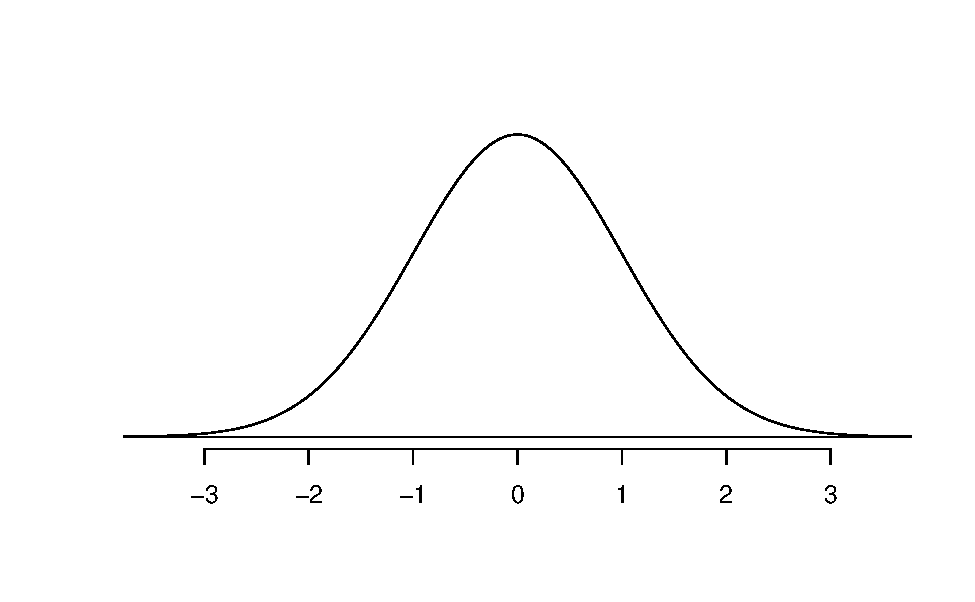
\includegraphics[width=0.5\linewidth]{04-A07-inference-1cat-theory_files/figure-latex/Normcur-1} 

}

\caption{Standard Normal Curve}\label{fig:Normcur}
\end{figure}

\begin{enumerate}
\def\labelenumi{\arabic{enumi}.}
\setcounter{enumi}{5}
\tightlist
\item
  Using the null standard error of the sample proportion, calculate the standardized sample proportion (Z). Mark this value on the standard normal distribution above.
\end{enumerate}

\vspace{0.6in}

The standardized statistic is used as a ruler to measure how far the sample statistic is from the null value. Essentially, we are converting the sample proportion into a measure of standard errors to compare to the standard normal distribution.

The standardized statistic measures the \emph{number of standard errors the sample statistic is from the null value}.

** Interpretation of the standardized sample proportion:**

\vspace{.8in}

We will use the \texttt{pnorm()} function in \texttt{R} to find the p-value. In the code below, notice that we used \texttt{lower.tail\ =\ FALSE} to find the p-value. \texttt{R} will calculate the p-value \emph{greater} than the value of the standardized statistic.

Notes:

\begin{itemize}
\tightlist
\item
  Use \texttt{lower.tail\ =\ TRUE} when doing a left-sided test.
\item
  Use \texttt{lower.tail\ =\ FALSE} when doing a right-sided test.
\item
  To find a two-sided p-value, use a left-sided test for negative Z or a right-sided test for positive Z, then multiply the value found by 2 to get the p-value.
\end{itemize}

\begin{Shaded}
\begin{Highlighting}[]
\FunctionTok{pnorm}\NormalTok{(}\FloatTok{4.769}\NormalTok{, }\CommentTok{\# Enter value of standardized statistic}
      \AttributeTok{m=}\DecValTok{0}\NormalTok{, }\AttributeTok{s=}\DecValTok{1}\NormalTok{, }\CommentTok{\# Using the standard normal mean = 0, sd = 1}
      \AttributeTok{lower.tail=}\ConstantTok{FALSE}\NormalTok{) }\CommentTok{\# Gives a p{-}value greater than the standardized statistic}
\end{Highlighting}
\end{Shaded}

\begin{enumerate}
\def\labelenumi{\arabic{enumi}.}
\setcounter{enumi}{6}
\item
  Report the p-value obtained from the \texttt{R} output.
  \vspace{0.3in}
\item
  Write a conclusion based on the p-value.
\end{enumerate}

\vspace{0.6in}

\begin{enumerate}
\def\labelenumi{\arabic{enumi}.}
\setcounter{enumi}{8}
\tightlist
\item
  To what group of observational units can the results be generalized to.
\end{enumerate}

\vspace{0.4in}

\subsection*{Impacts on the P-value}\label{impacts-on-the-p-value}
\addcontentsline{toc}{subsection}{Impacts on the P-value}

Suppose that we want to show that the true proportion of male boxers \textbf{differs} from that in the general population.

\begin{enumerate}
\def\labelenumi{\arabic{enumi}.}
\setcounter{enumi}{9}
\tightlist
\item
  Write out the alternative hypothesis in notation for this new research question.
\end{enumerate}

\vspace{0.3in}

\begin{figure}

{\centering 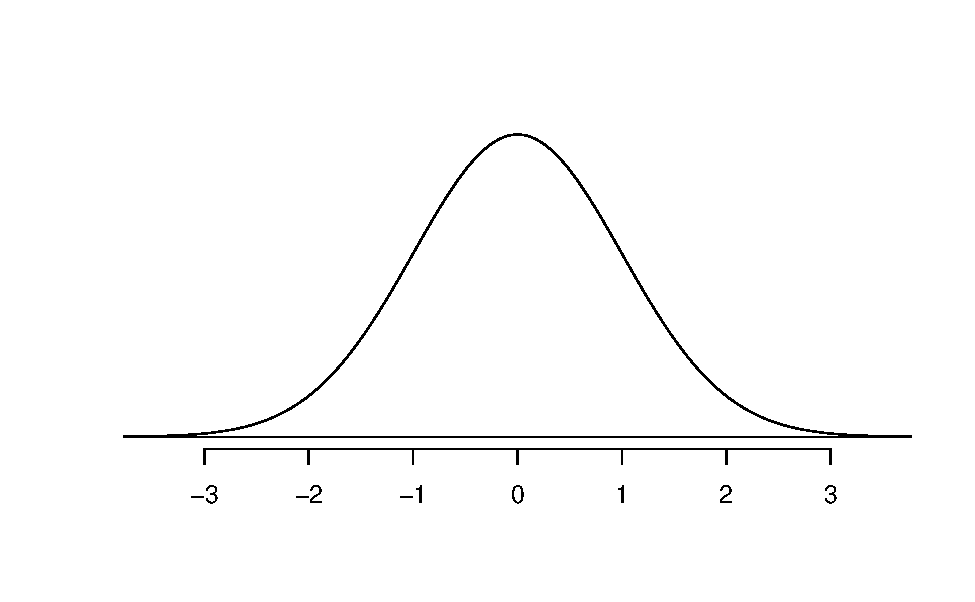
\includegraphics[width=0.5\linewidth]{04-A07-inference-1cat-theory_files/figure-latex/Norm-1} 

}

\caption{Standard Normal Curve}\label{fig:Norm}
\end{figure}

\begin{enumerate}
\def\labelenumi{\arabic{enumi}.}
\setcounter{enumi}{10}
\tightlist
\item
  How would this impact the p-value? Would the p-value be larger or smaller?
\end{enumerate}

\vspace{0.2in}

Suppose instead of 500 male boxers the researchers only took a sample of 300 male boxers and found the same proportion (\(\hat{p}=0.162\)) of male boxers that are left-handed. Since we are still assuming the same null value, 0.1, the standard error would be calculated as below:

\[SE_0(\hat{p})=\sqrt{\frac{0.1(1-0.1)}{300}} = 0.017\].

The standardized statistic for this new sample is calculated below:

\[Z = \frac{0.162-0.1}{0.017} = 3.64\]

\begin{figure}

{\centering 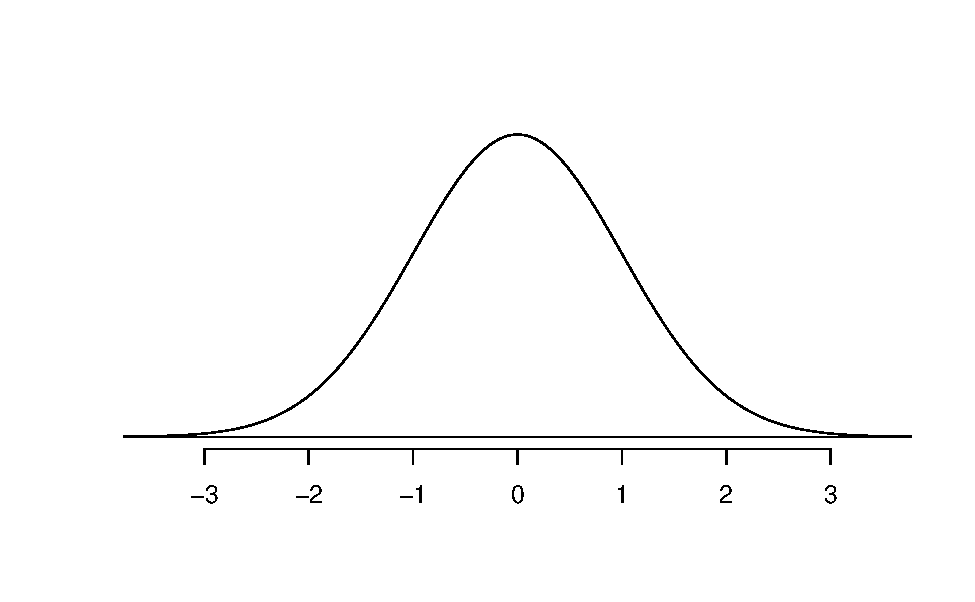
\includegraphics[width=0.5\linewidth]{04-A07-inference-1cat-theory_files/figure-latex/Norcur-1} 

}

\caption{Standard Normal Curve}\label{fig:Norcur}
\end{figure}

\begin{enumerate}
\def\labelenumi{\arabic{enumi}.}
\setcounter{enumi}{11}
\tightlist
\item
  How does the decrease in sample size affect the p-value?
\end{enumerate}

\vspace{0.3in}

Suppose another sample of 500 male boxers was taken and 68 were found to be left-handed. Since we are still assuming the same null value, 0.1, the standard error would be calculated as before:

\[SE_0(\hat{p})=\sqrt{\frac{0.1(1-0.1)}{500}} = 0.013\].

The standardized statistic for this new sample is calculated below:

\[Z = \frac{0.136-0.1}{0.013} = 2.769\]

\begin{figure}

{\centering 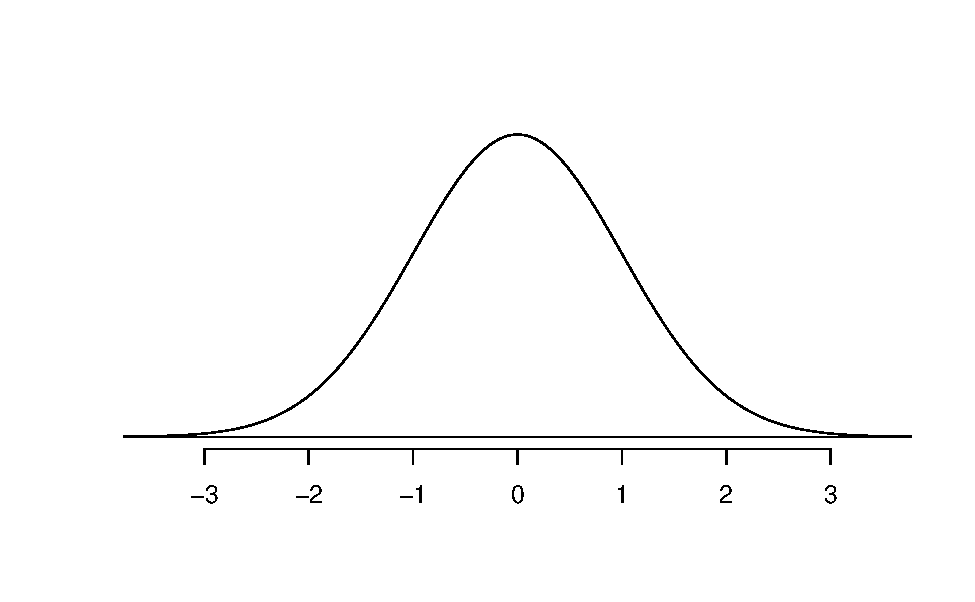
\includegraphics[width=0.5\linewidth]{04-A07-inference-1cat-theory_files/figure-latex/Norcuv-1} 

}

\caption{Standard Normal Curve}\label{fig:Norcuv}
\end{figure}

\begin{enumerate}
\def\labelenumi{\arabic{enumi}.}
\setcounter{enumi}{12}
\tightlist
\item
  How does a statistic closer to the null value affect the p-value?
\end{enumerate}

\vspace{0.3in}

\begin{enumerate}
\def\labelenumi{\arabic{enumi}.}
\setcounter{enumi}{13}
\tightlist
\item
  Summarize how each of the following affected the p-value:
\end{enumerate}

\begin{enumerate}
\def\labelenumi{\alph{enumi})}
\tightlist
\item
  Switching to a two-sided test.
\end{enumerate}

\vspace{0.4in}

\begin{enumerate}
\def\labelenumi{\alph{enumi})}
\setcounter{enumi}{1}
\tightlist
\item
  Using a smaller sample size.
\end{enumerate}

\vspace{0.4in}

\begin{enumerate}
\def\labelenumi{\alph{enumi})}
\setcounter{enumi}{2}
\tightlist
\item
  Using a sample statistic closer to the null value.
\end{enumerate}

\vspace{0.4in}

\subsection{Take-home messages}\label{take-home-messages-6}

\begin{enumerate}
\def\labelenumi{\arabic{enumi}.}
\item
  Both simulation and theory-based methods can be used to find a p-value for a hypothesis test. In order to use theory-based methods we need to check that both the independence and the success-failure conditions are met.
\item
  The standardized statistic measures how many standard errors the statistic is from the null value. The larger the standardized statistic the more evidence there is against the null hypothesis.
\item
  The p-value for a two-sided test is approximately two times the value for a one-sided test. A two-sided test provides less evidence against the null hypothesis.
\item
  The larger the sample size, the smaller the sample to sample variability. This will result in a larger standardized statistic and more evidence against the null hypothesis.
\item
  The farther the statistic is from the null value, the larger the standardized statistic. This will result in a smaller p-value and more evidence against the null hypothesis.
\end{enumerate}

\subsection{Additional notes}\label{additional-notes-6}

Use this space to summarize your thoughts and take additional notes on today's activity and material covered.

\newpage

\section{Activity 8: Confidence interval and what confidence means}\label{activity-8-confidence-interval-and-what-confidence-means}

\setstretch{1}

\subsection{Learning outcomes}\label{learning-outcomes-7}

\begin{itemize}
\item
  Explore what confidence means
\item
  Interpret the confidence level
\item
  Explore impact of sample size, direction of the alternative hypothesis, and value of the sample statistic on the p-value.
\end{itemize}

\subsection{Terminology review}\label{terminology-review-6}

In this activity, we will explore what being 95\% confidence means. Some terms covered in this activity are:

\begin{itemize}
\item
  Parameter of interest
\item
  Two-sided vs.~one-sided tests
\item
  Confidence level
\end{itemize}

\subsection{Handedness of male boxers continued}\label{handedness-of-male-boxers-continued}

In today's activity, we will use the male boxer study to look at what confidence means.

Left-handedness is a trait that is found in about 10\% of the general population. Past studies have shown that left-handed men are over-represented among professional boxers (Richardson and Gilman 2019). Is there evidence that there is an over-prevalence of left-handed fighters? In this random sample of 500 professional male boxers, 81 were left-handed.

\begin{Shaded}
\begin{Highlighting}[]
 \CommentTok{\# Read in data set}
\NormalTok{boxers }\OtherTok{\textless{}{-}} \FunctionTok{read.csv}\NormalTok{(}\StringTok{"https://math.montana.edu/courses/s216/data/Male\_boxers\_sample.csv"}\NormalTok{)}
\NormalTok{boxers }\SpecialCharTok{\%\textgreater{}\%} \FunctionTok{count}\NormalTok{(Stance)  }\CommentTok{\# Count number in each Stance category}
\end{Highlighting}
\end{Shaded}

\begin{verbatim}
#>         Stance   n
#> 1  left-handed  81
#> 2 right-handed 419
\end{verbatim}

\subsection*{\texorpdfstring{What does \emph{confidence} mean?}{What does confidence mean?}}\label{what-does-confidence-mean}
\addcontentsline{toc}{subsection}{What does \emph{confidence} mean?}

In the interpretation of a 95\% confidence interval, we say that we are 95\% confident that the parameter is within the confidence interval. Why are we able to make that claim? What does it mean to say ``we are 95\% confident''?

\begin{enumerate}
\def\labelenumi{\arabic{enumi}.}
\tightlist
\item
  In the last activity we found very strong evidence that the true proportion of male professional boxers that are left-handed is greater than 0.1. As a class, determine a plausible value for the true proportion of male boxers that are left-handed. \emph{Note: we are making assumptions about the population here. This is not based on our calculated data, but we will use this applet to better understand what happens when we take many, many samples from this believed population.}
\end{enumerate}

\vspace{0.2in}

\begin{enumerate}
\def\labelenumi{\arabic{enumi}.}
\setcounter{enumi}{1}
\tightlist
\item
  Go to this website, \url{http://www.rossmanchance.com/ISIapplets.html} and choose `Simulating Confidence Intervals'. In the input on the left-hand side of the screen enter the value from question 1 for \(\pi\) (the true value), 500 for \(n\), and 100 for `Number of intervals'. Click `sample'.
\end{enumerate}

\vspace{1mm}

\begin{itemize}
\tightlist
\item
  In the graph on the bottom right, click on a green dot. Write down the confidence interval for this sample given on the graph on the left. Does this confidence interval contain the true value chosen in question 1?
\end{itemize}

\vspace{0.4in}

\begin{itemize}
\item
  Now click on a red dot. Write down the confidence interval for this sample. Does this confidence interval contain the true value chosen in question 1?
  \vspace{0.5in}
\item
  How many intervals out of 100 contain \(\pi\), the true value chosen in question 1? \emph{Hint}: This is given to the left of the graph of green and red intervals.
  \vspace{0.4in}
\end{itemize}

\begin{enumerate}
\def\labelenumi{\arabic{enumi}.}
\setcounter{enumi}{2}
\tightlist
\item
  Click on `sample' nine more times. Write down the `Running Total' for the proportion of intervals that contain \(\pi\).
\end{enumerate}

\vspace{0.5in}

\begin{enumerate}
\def\labelenumi{\arabic{enumi}.}
\setcounter{enumi}{3}
\tightlist
\item
  Change the confidence level to 90\%. What happened to the width of the intervals?
\end{enumerate}

\vspace{0.2in}

\begin{enumerate}
\def\labelenumi{\arabic{enumi}.}
\setcounter{enumi}{4}
\tightlist
\item
  Write down the \texttt{Running\ Total} for the proportion of intervals that contain \(\pi\) using a 90\% confidence level.
\end{enumerate}

\vspace{0.4in}

\textbf{Interpretation of the level of confidence:}

\vspace{0.8in}

\subsubsection*{Notes on theory-based confidence intervals}\label{notes-on-theory-based-confidence-intervals}
\addcontentsline{toc}{subsubsection}{Notes on theory-based confidence intervals}

To calculate a theory-based 95\% confidence interval for \(\pi\), we will first find the \textbf{standard error} of \(\hat{p}\) by plugging in the value of \(\hat{p}\) for \(\pi\) in \(SD(\hat{p})\):

\[SE(\hat{p}) = \sqrt{\frac{\hat{p}\times (1-\hat{p})}{n}}\]

Note that we do not include a ``0'' subscript, since we are not assuming a null hypothesis.

\textbf{Calculate the standard error of the sample proportion to find a 95\% confidence interval.}

\vspace{0.5in}

We will calculate the margin of error and confidence interval later in this activity. \textbf{The margin of error (ME)} is the value of the \(z^*\) multiplier times the standard error of the statistic.

\[ME = z^* \times SE(\hat{p})\]
The \(z^*\) multiplier is the percentile of a standard normal distribution that corresponds to our confidence level. If our confidence level is 95\%, we find the Z values that encompass the middle 95\% of the standard normal distribution. If 95\% of the standard normal distribution should be in the middle, that leaves 5\% in the tails, or 2.5\% in each tail.

The \texttt{qnorm()} function in R will tell us the \(z^*\) value for the desired percentile (in this case, 95\% + 2.5\% = 97.5\% percentile).

\begin{figure}

{\centering 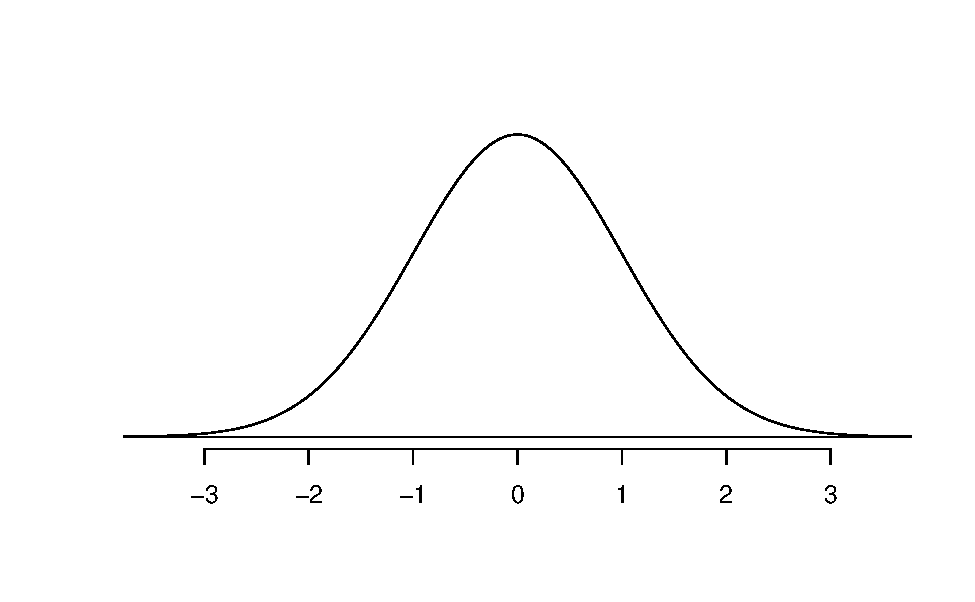
\includegraphics[width=0.45\linewidth]{04-A08-confidenceLevel_files/figure-latex/Normalcur-1} 

}

\caption{Standard Normal Curve}\label{fig:Normalcur}
\end{figure}

The following code will find the \(z^*\) value for a 95\% confidence interval.

\begin{Shaded}
\begin{Highlighting}[]
\FunctionTok{qnorm}\NormalTok{(}\FunctionTok{c}\NormalTok{(}\FloatTok{0.025}\NormalTok{, }\FloatTok{0.975}\NormalTok{), }\AttributeTok{lower.tail =} \ConstantTok{TRUE}\NormalTok{) }\CommentTok{\# Multiplier for 95\% confidence interval}
\end{Highlighting}
\end{Shaded}

\textbf{Calculate the margin of error for the 95\% confidence interval.}
\vspace{0.6in}

To find the confidence interval, we will add and subtract the \textbf{margin of error} to the point estimate:
\[\text{point estimate}\pm\text{margin of error}\]
\[\hat{p}\pm z^* \times SE(\hat{p})\]

\textbf{Calculate the 95\% confidence interval for the parameter of interest.}
\vspace{0.6in}

\begin{enumerate}
\def\labelenumi{\arabic{enumi}.}
\setcounter{enumi}{5}
\tightlist
\item
  Interpret the 95\% confidence \textbf{interval} in the context of the problem.
  \vspace{1in}
\end{enumerate}

\subsubsection*{Simulation methods}\label{simulation-methods}
\addcontentsline{toc}{subsubsection}{Simulation methods}

We could also use simulation-based methods to analyze these data.

\begin{center}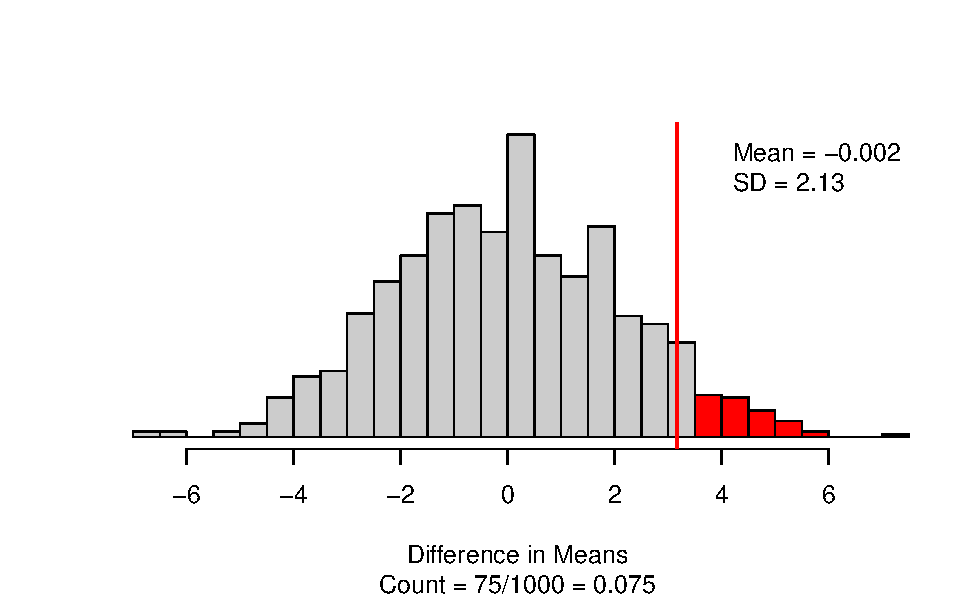
\includegraphics[width=0.7\linewidth]{04-A08-confidenceLevel_files/figure-latex/unnamed-chunk-3-1} \end{center}

\begin{center}\includegraphics[width=0.7\linewidth]{04-A08-confidenceLevel_files/figure-latex/unnamed-chunk-4-1} \end{center}

\begin{enumerate}
\def\labelenumi{\arabic{enumi}.}
\setcounter{enumi}{6}
\tightlist
\item
  Explain why the results for simulation methods and theory-based methods are similar.
\end{enumerate}

\vspace{1in}

\subsection{Take-home messages}\label{take-home-messages-7}

\begin{enumerate}
\def\labelenumi{\arabic{enumi}.}
\item
  If repeat samples of the same size are selected from the population, approximately 95\% of samples will create a 95\% confidence interval that contains the parameter of interest.
\item
  The calculation of the confidence interval uses the standard error calculated using the sample proportion rather than the null value.
\end{enumerate}

\subsection{Additional notes}\label{additional-notes-7}

Use this space to summarize your thoughts and take additional notes on today's activity and material covered.

\newpage

\section{Module 3 and 4 Lab: Mixed Breed Dogs in the U.S.}\label{module-3-and-4-lab-mixed-breed-dogs-in-the-u.s.}

\setstretch{1}

\subsection{Learning outcomes}\label{learning-outcomes-8}

\begin{itemize}
\item
  Determine whether simulation or theory-based methods of inference can be used.
\item
  Analyze and interpret a study involving a single categorical variable.
\end{itemize}

\subsection{Mixed Breed Dogs in the U.S.}\label{mixed-breed-dogs-in-the-u.s.}

The American Veterinary Medical Association estimated in 2010 that approximately 49\% of dog owners in the U.S. own dogs that are classified as ``mixed breed.'' As part of a larger 2022 international study (Banton 2022) about overall dog health, survey participants were asked, among other things, to report whether their dog was purebred or a mixed breed. Seven hundred and fifty (750) dog owners from the U.S. were recruited to complete an online survey via an email indicating they had been randomly selected by Qualtrics (an ``experience management'' company that specializes in surveys). Three hundred sixty-four (364) out of 675 respondents from the U.S. reported they owned a mixed breed dog. Is there evidence that, in the last decade, the proportion of dog owners in the U.S. that own a mixed breed dog has changed from the value reported in 2010?

\begin{itemize}
\item
  Observational units:
\item
  Variable:
\item
  Type of variable:
\item
  Success:
\end{itemize}

\subsubsection*{Activity intro}\label{activity-intro-1}
\addcontentsline{toc}{subsubsection}{Activity intro}

\begin{itemize}
\item
  Download the R script file and the data file (US\_dogs.csv) from D2L
\item
  Upload both files to D2L and open the R script file
\item
  Enter the name of the dataset for datasetname.csv.
\item
  Highlight and run lines 1 - 6
\end{itemize}

\begin{enumerate}
\def\labelenumi{\arabic{enumi}.}
\tightlist
\item
  What is the value of the point estimate?
\end{enumerate}

\vspace{0.3in}

\begin{enumerate}
\def\labelenumi{\arabic{enumi}.}
\setcounter{enumi}{1}
\tightlist
\item
  Create a plot of the data using the R code. Make sure to include an appropriate title with type of plot, observational units, and variable.
\end{enumerate}

\begin{Shaded}
\begin{Highlighting}[]
\NormalTok{dogs }\SpecialCharTok{\%\textgreater{}\%} \CommentTok{\# Data set piped into...}
    \FunctionTok{ggplot}\NormalTok{(}\FunctionTok{aes}\NormalTok{(}\AttributeTok{x =}\NormalTok{ variable)) }\SpecialCharTok{+}   \CommentTok{\# This specifies the variable}
    \FunctionTok{geom\_bar}\NormalTok{(}\FunctionTok{aes}\NormalTok{(}\AttributeTok{y =} \FunctionTok{after\_stat}\NormalTok{(prop), }\AttributeTok{group =} \DecValTok{1}\NormalTok{)) }\SpecialCharTok{+}  \CommentTok{\# Tell it to make a bar plot with proportions}
    \FunctionTok{labs}\NormalTok{(}\AttributeTok{title =} \StringTok{"Don\textquotesingle{}t forget to title your plot"}\NormalTok{,  }
       \CommentTok{\# Give your plot a title}
       \AttributeTok{x =} \StringTok{"Breed of Dog"}\NormalTok{,   }\CommentTok{\# Label the x axis}
       \AttributeTok{y =} \StringTok{"Relative Frequency"}\NormalTok{)  }\CommentTok{\# Label the y axis}
\end{Highlighting}
\end{Shaded}

\subsubsection*{Use statistical analysis methods to draw inferences from the data}\label{use-statistical-analysis-methods-to-draw-inferences-from-the-data-2}
\addcontentsline{toc}{subsubsection}{Use statistical analysis methods to draw inferences from the data}

\begin{enumerate}
\def\labelenumi{\arabic{enumi}.}
\setcounter{enumi}{2}
\tightlist
\item
  Write out the parameter of interest in words, in context of the study.
\end{enumerate}

\vspace{0.5in}

\begin{enumerate}
\def\labelenumi{\arabic{enumi}.}
\setcounter{enumi}{3}
\tightlist
\item
  Write out the null and alternative hypotheses in notation.
\end{enumerate}

\vspace{1mm}

\(H_0:\)

\vspace{0.3in}

\(H_A:\)

\vspace{0.3in}

\begin{enumerate}
\def\labelenumi{\arabic{enumi}.}
\setcounter{enumi}{4}
\tightlist
\item
  Will theory-based methods give the same results as simulation based methods? Explain your answer.
\end{enumerate}

\vspace{1in}

\subsubsection*{Null Distribution}\label{null-distribution}
\addcontentsline{toc}{subsubsection}{Null Distribution}

To use the computer simulation, we will need to enter the

\begin{itemize}
\item
  assumed ``probability of success'' (\(\pi_0\)),
\item
  ``sample size'' (the number of observational units or cases in the sample),
\item
  ``number of repetitions'' (the number of samples to be generated),
\item
  ``as extreme as'' (the observed statistic), and
\item
  the ``direction'' (matches the direction of the alternative hypothesis).
\end{itemize}

We will use the \texttt{one\_proportion\_test()} function in \texttt{R} (in the \texttt{catstats} package) to simulate the null distribution of sample proportions and compute a p-value.

\begin{itemize}
\item
  Using the provided \texttt{R} script file, fill in the values/words for each \texttt{xx} in the one proportion test to create a null distribution with 10000 simulations.
\item
  Then highlight and run lines 21--26.
\end{itemize}

\begin{Shaded}
\begin{Highlighting}[]
\FunctionTok{one\_proportion\_test}\NormalTok{(}\AttributeTok{probability\_success =}\NormalTok{ xx, }\CommentTok{\# Null hypothesis value}
          \AttributeTok{sample\_size =}\NormalTok{ xx, }\CommentTok{\# Enter sample size}
          \AttributeTok{number\_repetitions =} \DecValTok{10000}\NormalTok{, }\CommentTok{\# Enter number of simulations}
          \AttributeTok{as\_extreme\_as =}\NormalTok{ xx, }\CommentTok{\# Observed statistic}
          \AttributeTok{direction =} \StringTok{"xx"}\NormalTok{, }\CommentTok{\# Specify direction of alternative hypothesis}
          \AttributeTok{summary\_measure =} \StringTok{"proportion"}\NormalTok{) }\CommentTok{\# Reporting proportion or number of successes?}
\end{Highlighting}
\end{Shaded}

\begin{enumerate}
\def\labelenumi{\arabic{enumi}.}
\setcounter{enumi}{5}
\tightlist
\item
  Report the p-value from the study.
\end{enumerate}

\vspace{0.2in}

\subsubsection*{Bootstrap distribution}\label{bootstrap-distribution}
\addcontentsline{toc}{subsubsection}{Bootstrap distribution}

We will use the \texttt{one\_proportion\_bootstrap\_CI()} function in R (in the \texttt{catstats} package) to simulate the bootstrap distribution of sample proportions and calculate a confidence interval. Using the provided R script file, fill in the values/words for each \texttt{xx} in the one proportion bootstrap confidence interval (CI) code to create a bootstrap distribution with 10000 simulations. Then highlight and run lines ??? to create a 90\% confidence interval.

\begin{Shaded}
\begin{Highlighting}[]
\FunctionTok{one\_proportion\_bootstrap\_CI}\NormalTok{(}\AttributeTok{sample\_size =}\NormalTok{ xx, }\CommentTok{\# Sample size}
                    \AttributeTok{number\_successes =}\NormalTok{ xx, }\CommentTok{\# Observed number of successes}
                    \AttributeTok{number\_repetitions =} \DecValTok{10000}\NormalTok{, }\CommentTok{\# Number of bootstrap samples to use}
                    \AttributeTok{confidence\_level =}\NormalTok{ xx) }\CommentTok{\# Confidence level as a decimal}
\end{Highlighting}
\end{Shaded}

\begin{enumerate}
\def\labelenumi{\arabic{enumi}.}
\setcounter{enumi}{6}
\tightlist
\item
  Report the 90\% confidence interval.
\end{enumerate}

\vspace{0.2in}

\subsubsection*{Summarize the results of the study}\label{summarize-the-results-of-the-study}
\addcontentsline{toc}{subsubsection}{Summarize the results of the study}

\begin{enumerate}
\def\labelenumi{\arabic{enumi}.}
\setcounter{enumi}{7}
\tightlist
\item
  Write a paragraph summarizing the results of the study. Be sure to describe:
\end{enumerate}

\begin{itemize}
\item
  Summary statistic and interpretation

  \begin{itemize}
  \item
    Summary measure (in context)
  \item
    Value of the statistic
  \item
    Order of subtraction when comparing two groups
  \end{itemize}
\item
  P-value and interpretation

  \begin{itemize}
  \item
    Statement about probability or proportion of samples
  \item
    Statistic (summary measure and value)
  \item
    Direction of the alternative
  \item
    Null hypothesis (in context)
  \end{itemize}
\item
  Confidence interval and interpretation

  \begin{itemize}
  \item
    How confident you are (e.g., 90\%, 95\%, 98\%, 99\%)
  \item
    Parameter of interest
  \item
    Calculated interval
  \item
    Order of subtraction when comparing two groups
  \end{itemize}
\item
  Conclusion (written to answer the research question)

  \begin{itemize}
  \item
    Amount of evidence
  \item
    Parameter of interest
  \item
    Direction of the alternative hypothesis
  \end{itemize}
\item
  Scope of inference

  \begin{itemize}
  \item
    To what group of observational units do the results apply (target population or observational units similar to the sample)?
  \item
    What type of inference is appropriate (causal or non-causal)?
  \end{itemize}
\end{itemize}

\textbf{Upload a copy of your group's paragraph to Gradescope.}

\newpage

Paragraph (continued):

\newpage

\phantomsection\label{refs}
\begin{CSLReferences}{1}{0}
\bibitem[\citeproctext]{ref-pga}
{``Average Driving Distance and Fairway Accuracy.''} 2008. \href{https://www.pga.com/\%20and\%20https://www.lpga.com/}{https://www.pga.com/ and https://www.lpga.com/}.

\bibitem[\citeproctext]{ref-banton2022}
Banton, et al, S. 2022. {``Jog with Your Dog: Dog Owner Exercise Routines Predict Dog Exercise Routines and Perception of Ideal Body Weight.''} \emph{PLoS ONE} 17(8).

\bibitem[\citeproctext]{ref-bhavsar2022}
Bhavsar, et al, A. 2022. {``Increased Risk of Herpes Zoster in Adults \(\geq\)50 Years Old Diagnosed with COVID-19 in the United States.''} \emph{Open Forum Infectious Diseases} 9(5).

\bibitem[\citeproctext]{ref-islands}
Bulmer, M. n.d. {``Islands in Schools Project.''} \url{https://sites.google.com/site/islandsinschoolsprojectwebsite/home}.

\bibitem[\citeproctext]{ref-bts}
{``Bureau of Transportation Statistics.''} 2019. \url{https://www.bts.gov/}.

\bibitem[\citeproctext]{ref-babies}
{``Child Health and Development Studies.''} n.d. \url{https://www.chdstudies.org/}.

\bibitem[\citeproctext]{ref-darley1973}
Darley, J. M., and C. D. Batson. 1973. {``"From Jerusalem to Jericho": A Study of Situational and Dispositional Variables in Helping Behavior.''} \emph{Journal of Personality and Social Psychology} 27: 100--108.

\bibitem[\citeproctext]{ref-davis2020}
Davis, Smith, A. K. 2020. {``A Poor Substitute for the Real Thing: Captive-Reared Monarch Butterflies Are Weaker, Paler and Have Less Elongated Wings Than Wild Migrants.''} \emph{Biology Letters} 16.

\bibitem[\citeproctext]{ref-doit2015}
Du Toit, et al, G. 2015. {``Randomized Trial of Peanut Consumption in Infants at Risk for Peanut Allergy.''} \emph{New England Journal of Medicine} 372.

\bibitem[\citeproctext]{ref-edmunds2016}
Edmunds, et al, D. 2016. {``Chronic Wasting Disease Drives Population Decline of White-Tailed Deer.''} \emph{PLoS ONE} 11(8).

\bibitem[\citeproctext]{ref-ipeds}
Education Statistics, National Center for. 2018. {``IPEDS.''} \url{https://nces.ed.gov/ipeds/}.

\bibitem[\citeproctext]{ref-gbmarried}
{``Great Britain Married Couples: Great Britain Office of Population Census and Surveys.''} n.d. \url{https://discovery.nationalarchives.gov.uk/details/r/C13351}.

\bibitem[\citeproctext]{ref-zeitler2012}
Group, TODAY Study. 2012. {``\href{https://www.ncbi.nlm.nih.gov/pubmed/22540912}{A Clinical Trial to Maintain Glycemic Control in Youth with Type 2 Diabetes}.''} \emph{New England Journal of Medicine} 366: 2247--56.

\bibitem[\citeproctext]{ref-hamblin2007}
Hamblin, J. K., K. Wynn, and P. Bloom. 2007. {``Social Evaluation by Preverbal Infants.''} \emph{Nature} 450 (6288): 557--59.

\bibitem[\citeproctext]{ref-hirschfelder2018}
Hirschfelder, A., and P. F. Molin. 2018. {``I Is for Ignoble: Stereotyping Native Americans.''} \href{Retrieved\%20from\%20https://www.ferris.edu/HTMLS/news/jimcrow/native/homepage.htm.}{Retrieved from https://www.ferris.edu/HTMLS/news/jimcrow/native/homepage.htm.}

\bibitem[\citeproctext]{ref-hutchison2013}
Hutchison, R. L., and M. A. Hirthler. 2013. {``\href{https://www.ncbi.nlm.nih.gov/pubmed/23932117}{Upper Extremity Injuies in Homer's Iliad}.''} \emph{Journal of Hand Surgery (American Volume)} 38: 1790--93.

\bibitem[\citeproctext]{ref-imdb}
{``{IMDb} Movies Extensive Dataset.''} 2016. \url{https://kaggle.com/stefanoleone992/imdb-extensive-dataset}.

\bibitem[\citeproctext]{ref-kalra2022}
Kalra, et al., Dl. 2022. {``Trustworthiness of Indian Youtubers.''} Kaggle. \url{https://doi.org/10.34740/KAGGLE/DSV/4426566}.

\bibitem[\citeproctext]{ref-keating2021}
Keating, D., N. Ahmed, F. Nirappil, Stanley-Becker I., and L. Bernstein. 2021. {``Coronavirus Infections Dropping Where People Are Vaccinated, Rising Where They Are Not, Post Analysis Finds.''} \emph{Washington Post}. \url{https://www.washingtonpost.com/health/2021/06/14/covid-cases-vaccination-rates/}.

\bibitem[\citeproctext]{ref-laeng2007}
Laeng, Mathisen, B. 2007. {``Why Do Blue-Eyed Men Prefer Women with the Same Eye Color?''} \emph{Behavioral Ecology and Sociobiology} 61(3).

\bibitem[\citeproctext]{ref-levin2000}
Levin, D. T. 2000. {``Race as a Visual Feature: Using Visual Search and Perceptual Discrimination Tasks to Understand Face Categories and the Cross-Race Recognition Deficit.''} \emph{Journal of Experimental Psychology} 129(4).

\bibitem[\citeproctext]{ref-luetkemeier2017}
LUETKEMEIER, et al., M. 2017. {``Skin Tattoos Alter Sweat Rate and Na+ Concentration.''} \emph{Medicine and Science in Sports and Exercise} 49(7).

\bibitem[\citeproctext]{ref-madden2020}
Madden, et al, J. 2020. {``Ready Student One: Exploring the Predictors of Student Learning in Virtual Reality.''} \emph{PLoS ONE} 15(3).

\bibitem[\citeproctext]{ref-miller1956}
Miller, G. A. 1956. {``The Magical Number Seven, Plus or Minus Two: Some Limits on Our Capacity for Processing Information.''} \emph{Psychological Review} 63(2).

\bibitem[\citeproctext]{ref-becentispeech}
Moquin, W., and C. Van Doren. 1973. {``Great Documents in American Indian History.''} Praeger.

\bibitem[\citeproctext]{ref-pew2022}
{``More Americans Are Joining the 'Cashless' Economy.''} 2022. \url{https://www.pewresearch.org/short-reads/2022/10/05/more-americans-are-joining-the-cashless-economy/.}

\bibitem[\citeproctext]{ref-weather}
National Weather Service Corporate Image Web Team. n.d. {``National Weather Service -- {NWS} Billings.''} \url{https://w2.weather.gov/climate/xmacis.php?wfo=byz}.

\bibitem[\citeproctext]{ref-obrien2019}
O'Brien, Lynch, H. D. 2019. {``Crocodylian Head Width Allometry and Phylogenetic Prediction of Body Size in Extinct Crocodyliforms.''} \emph{Integrative Organismal Biology} 1.

\bibitem[\citeproctext]{ref-ocean}
{``Ocean Temperature and Salinity Study.''} n.d. \url{https://calcofi.org/}.

\bibitem[\citeproctext]{ref-WashPost2022}
{``Older People Who Get Covid Are at Increased Risk of Getting Shingles.''} 2022. \url{https://www.washingtonpost.com/health/2022/04/19/shingles-and-covid-over-50/.}

\bibitem[\citeproctext]{ref-physhealth}
{``Physician's Health Study.''} n.d. \url{https://phs.bwh.harvard.edu/}.

\bibitem[\citeproctext]{ref-porath2017}
Porath, Erez, C. 2017. {``Does Rudeness Really Matter? The Effects of Rudeness on Task Performance and Helpfulness.''} \emph{Academy of Management Journal} 50.

\bibitem[\citeproctext]{ref-quinn1999}
Quinn, G. E., C. H. Shin, M. G. Maguire, and R. A. Stone. 1999. {``Myopia and Ambient Lighting at Night.''} \emph{Nature} 399 (6732): 113--14. \url{https://doi.org/10.1038/20094}.

\bibitem[\citeproctext]{ref-ramachandran2007}
Ramachandran, V. 2007. {``3 Clues to Understanding Your Brain.''} \url{https://www.ted.com/talks/vs_ramachandran_3_clues_to_understanding_your_brain}.

\bibitem[\citeproctext]{ref-cdchospitalization}
{``Rates of Laboratory-Confimed COVID-19 Hospitalizations by Vaccination Status.''} 2021. CDC. \url{https://covid.cdc.gov/covid-data-tracker/\#covidnet-hospitalizations-vaccination}.

\bibitem[\citeproctext]{ref-richardson2019}
Richardson, T., and R. T. Gilman. 2019. {``Left-Handedness Is Associated with Greater Fighting Success in Humans.''} \emph{Scientific Reports} 9 (1): 15402. \url{https://doi.org/10.1038/s41598-019-51975-3}.

\bibitem[\citeproctext]{ref-stephens2020}
Stephens, R., and O. Robertson. 2020. {``Swearing as a Response to Pain: Assessing Hypoalgesic Effects of Novel "Swear" Words.''} \emph{Frontiers in Psychology} 11: 643--62.

\bibitem[\citeproctext]{ref-stewart2014}
Stewart, E. H., B. Davis, B. L. Clemans-Taylor, B. Littenberg, C. A. Estrada, and R. M. Centor. 2014. {``Rapid Antigen Group a Streptococcus Test to Diagnose Pharyngitis: A Systematic Review and Meta-Analysis''} 9 (11). \url{https://doi.org/10.1371/journal.pone.0111727}.

\bibitem[\citeproctext]{ref-stroop1935}
Stroop, J. R. 1935. {``Studies of Interference in Serial Verbal Reactions.''} \emph{Journal of Experimental Psychology} 18: 643--62.

\bibitem[\citeproctext]{ref-subach2022}
Subach, et al, A. 2022. {``Foraging Behaviour, Habitat Use and Population Size of the Desert Horned Viper in the Negev Desert.''} \emph{Soc.Open Sci} 9.

\bibitem[\citeproctext]{ref-sulheim2017}
Sulheim, S., A. Ekeland, I. Holme, and R. Bahr. 2017. {``Helmet Use and Risk of Head Injuries in Alpine Skiers and Snowboarders: Changes After an Interval of One Decade''} 51 (1): 44--50. \url{https://doi.org/10.1136/bjsports-2015-095798}.

\bibitem[\citeproctext]{ref-titanic}
{``Titanic.''} n.d. \url{http://www.encyclopedia-titanica.org}.

\bibitem[\citeproctext]{ref-covidvaccinetracker}
{``US COVID-19 Vaccine Tracker: See Your State's Progress.''} 2021. Mayo Clinic. \url{https://www.mayoclinic.org/coronavirus-covid-19/vaccine-tracker}.

\bibitem[\citeproctext]{ref-usepa2020}
US Environmental Protection Agency. n.d. {``Air Data -- Daily Air Quality Tracker.''} \url{https://www.epa.gov/outdoor-air-quality-data/air-data-daily-air-quality-tracker}.

\bibitem[\citeproctext]{ref-wahlstrom2014}
Wahlstrom, et al, K. 2014. {``Examining the Impact of Later School Start Times on the Health and Academic Performance of High School Students: A Multi-Site Study.''} \emph{Center for Applied Research and Educational Improvement}.

\bibitem[\citeproctext]{ref-watson2015}
Watson, et al., N. 2015. {``Recommended Amount of Sleep for a Heathy Adult: A Joint Consensus Statement of the American Academy of Sleep Medicine and Sleep Research Society.''} \emph{Sleep} 38(6).

\bibitem[\citeproctext]{ref-Weiss1988}
Weiss, R. D. 1988. {``Relapse to Cocaine Abuse After Initiating Desipramine Treatment.''} \emph{JAMA} 260(17).

\bibitem[\citeproctext]{ref-navajo2011}
{``Welcome to the Navajo Nation Government: Official Site of the Navajo Nation.''} 2011.\href{\%20Retrieved\%20from\%20https://www.navajo-nsn.gov/.}{Retrieved from https://www.navajo-nsn.gov/.}

\bibitem[\citeproctext]{ref-wilson2016}
Wilson, Woodruff, J. P. 2016. {``Vertebral Adaptations to Large Body Size in Theropod Dinosaurs.''} \emph{PLoS ONE} 11(7).

\end{CSLReferences}

\end{document}
